\chapter{Resultados experimentales}

\section{Métricas de evaluación y criterios de análisis}

La evaluación del rendimiento de los agentes de Aprendizaje por Refuerzo en el entorno \textit{SimplePacmanEnv} se ha realizado utilizando dos métricas principales: la recompensa media por episodio (\textit{mean reward}) y el ratio de completado del entorno (\textit{completion ratio}). Estas métricas capturan aspectos complementarios del comportamiento del agente y permiten un análisis más completo que el uso de una única medida agregada.

La recompensa media por episodio refleja el retorno acumulado obtenido por el agente durante un episodio, teniendo en cuenta tanto las recompensas positivas (recolección de monedas y finalización exitosa) como las penalizaciones (colisiones con el fantasma y coste temporal por paso). Esta métrica es especialmente útil para analizar la eficiencia del comportamiento aprendido, ya que penaliza trayectorias largas o ineficientes incluso cuando el agente logra recolectar una cantidad significativa de monedas.

Por otro lado, el \textit{completion ratio} mide la fracción de monedas recolectadas respecto al total disponible en el entorno durante un episodio. Esta métrica proporciona una medida directa del progreso del agente hacia el objetivo global de la tarea, independientemente de la duración del episodio o del coste temporal asociado. En este sentido, el \textit{completion ratio} permite evaluar hasta qué punto el agente es capaz de explorar el entorno y cubrir sus distintas regiones.

Es importante destacar que ambas métricas capturan comportamientos distintos y no siempre están correlacionadas. Por ejemplo, un agente puede maximizar la recompensa media adoptando una estrategia miope que priorice la recolección de monedas cercanas o seguras, evitando zonas de mayor riesgo. En este caso, el agente puede obtener un \textit{mean reward} elevado sin llegar a completar el entorno, lo que se reflejaría en un \textit{completion ratio} moderado o bajo.

De manera análoga, dos agentes pueden completar sistemáticamente el entorno y, por tanto, presentar valores similares de \textit{completion ratio}, pero diferir en su recompensa media. Esta situación puede darse cuando uno de los agentes resuelve la tarea de forma más eficiente, empleando menos pasos y evitando penalizaciones temporales innecesarias, lo que se traduce en un mayor \textit{mean reward}. En contraste, un agente que complete el entorno de forma más lenta o errática obtendrá una recompensa media inferior a pesar de alcanzar el mismo grado de completado.

Por este motivo, el análisis experimental presentado en este capítulo se apoya en ambas métricas de manera complementaria. El \textit{mean reward} se utiliza para evaluar la eficiencia y estabilidad del comportamiento aprendido, mientras que el \textit{completion ratio} permite medir el grado de cumplimiento del objetivo global de la tarea. La interpretación conjunta de ambas métricas resulta esencial para comprender adecuadamente el impacto de la complejidad del estado en el proceso de aprendizaje.

\section{Resultados por algoritmo}

En este capítulo se presentan los resultados obtenidos a partir de los experimentos descritos en el capítulo anterior. El objetivo es analizar el comportamiento de los distintos algoritmos de Aprendizaje por Refuerzo evaluados —DQN, A2C y PPO— bajo diferentes configuraciones de observación, manteniendo constantes las dinámicas del entorno y el sistema de recompensas.

Los resultados se han obtenido a partir de múltiples ejecuciones independientes, utilizando diferentes semillas aleatorias con el fin de reducir la variabilidad inherente al proceso de aprendizaje. Para cada configuración se han registrado métricas cuantitativas como la recompensa media por episodio, la duración media de los episodios y la estabilidad del entrenamiento, así como métricas derivadas de la evaluación periódica de los modelos entrenados.

Este apartado se centra en describir el comportamiento de cada algoritmo de forma individual, sin establecer todavía comparaciones directas entre ellos. El análisis comparativo se abordará en secciones posteriores, una vez presentados los resultados de cada método de manera aislada.

\subsection{Resultados con Deep Q-Network (DQN)}

En este apartado se presentan los resultados obtenidos con el algoritmo Deep Q-Network (DQN) bajo las distintas configuraciones de observación definidas en el entorno \textit{SimplePacmanEnv}. El objetivo es analizar el comportamiento del algoritmo de forma aislada, sin establecer aún comparaciones directas con otros métodos de aprendizaje por refuerzo.

Tras una fase inicial de ajuste manual, los hiperparámetros de DQN fueron optimizados mediante la librería Optuna utilizando 40 \textit{trials} y 300\,000 pasos de entrenamiento por prueba para cada modo de observación. Posteriormente, los modelos seleccionados fueron entrenados de manera más exhaustiva durante 5 millones de pasos, aplicando un protocolo de evaluación periódica con 75 episodios, una frecuencia de evaluación de 20\,000 pasos y un criterio de parada temprana. Finalmente, cada modelo fue evaluado sobre 100 episodios independientes para obtener métricas finales de rendimiento.

Los resultados muestran que DQN es capaz de aprender comportamientos parcialmente efectivos en el entorno, con un rendimiento muy dependiente del modo de observación. En particular, el modo \textit{coins\_quadrants} presenta la recompensa media más elevada (41.81), seguido por \textit{power\_time} (37.18) y \textit{bool\_power} (31.22). En contraste, el modo de observación mínima obtiene una recompensa media negativa (-14.56), lo que sugiere que una representación excesivamente simplificada dificulta el aprendizaje de políticas útiles en este entorno.

\begin{figure}[h]
\centering
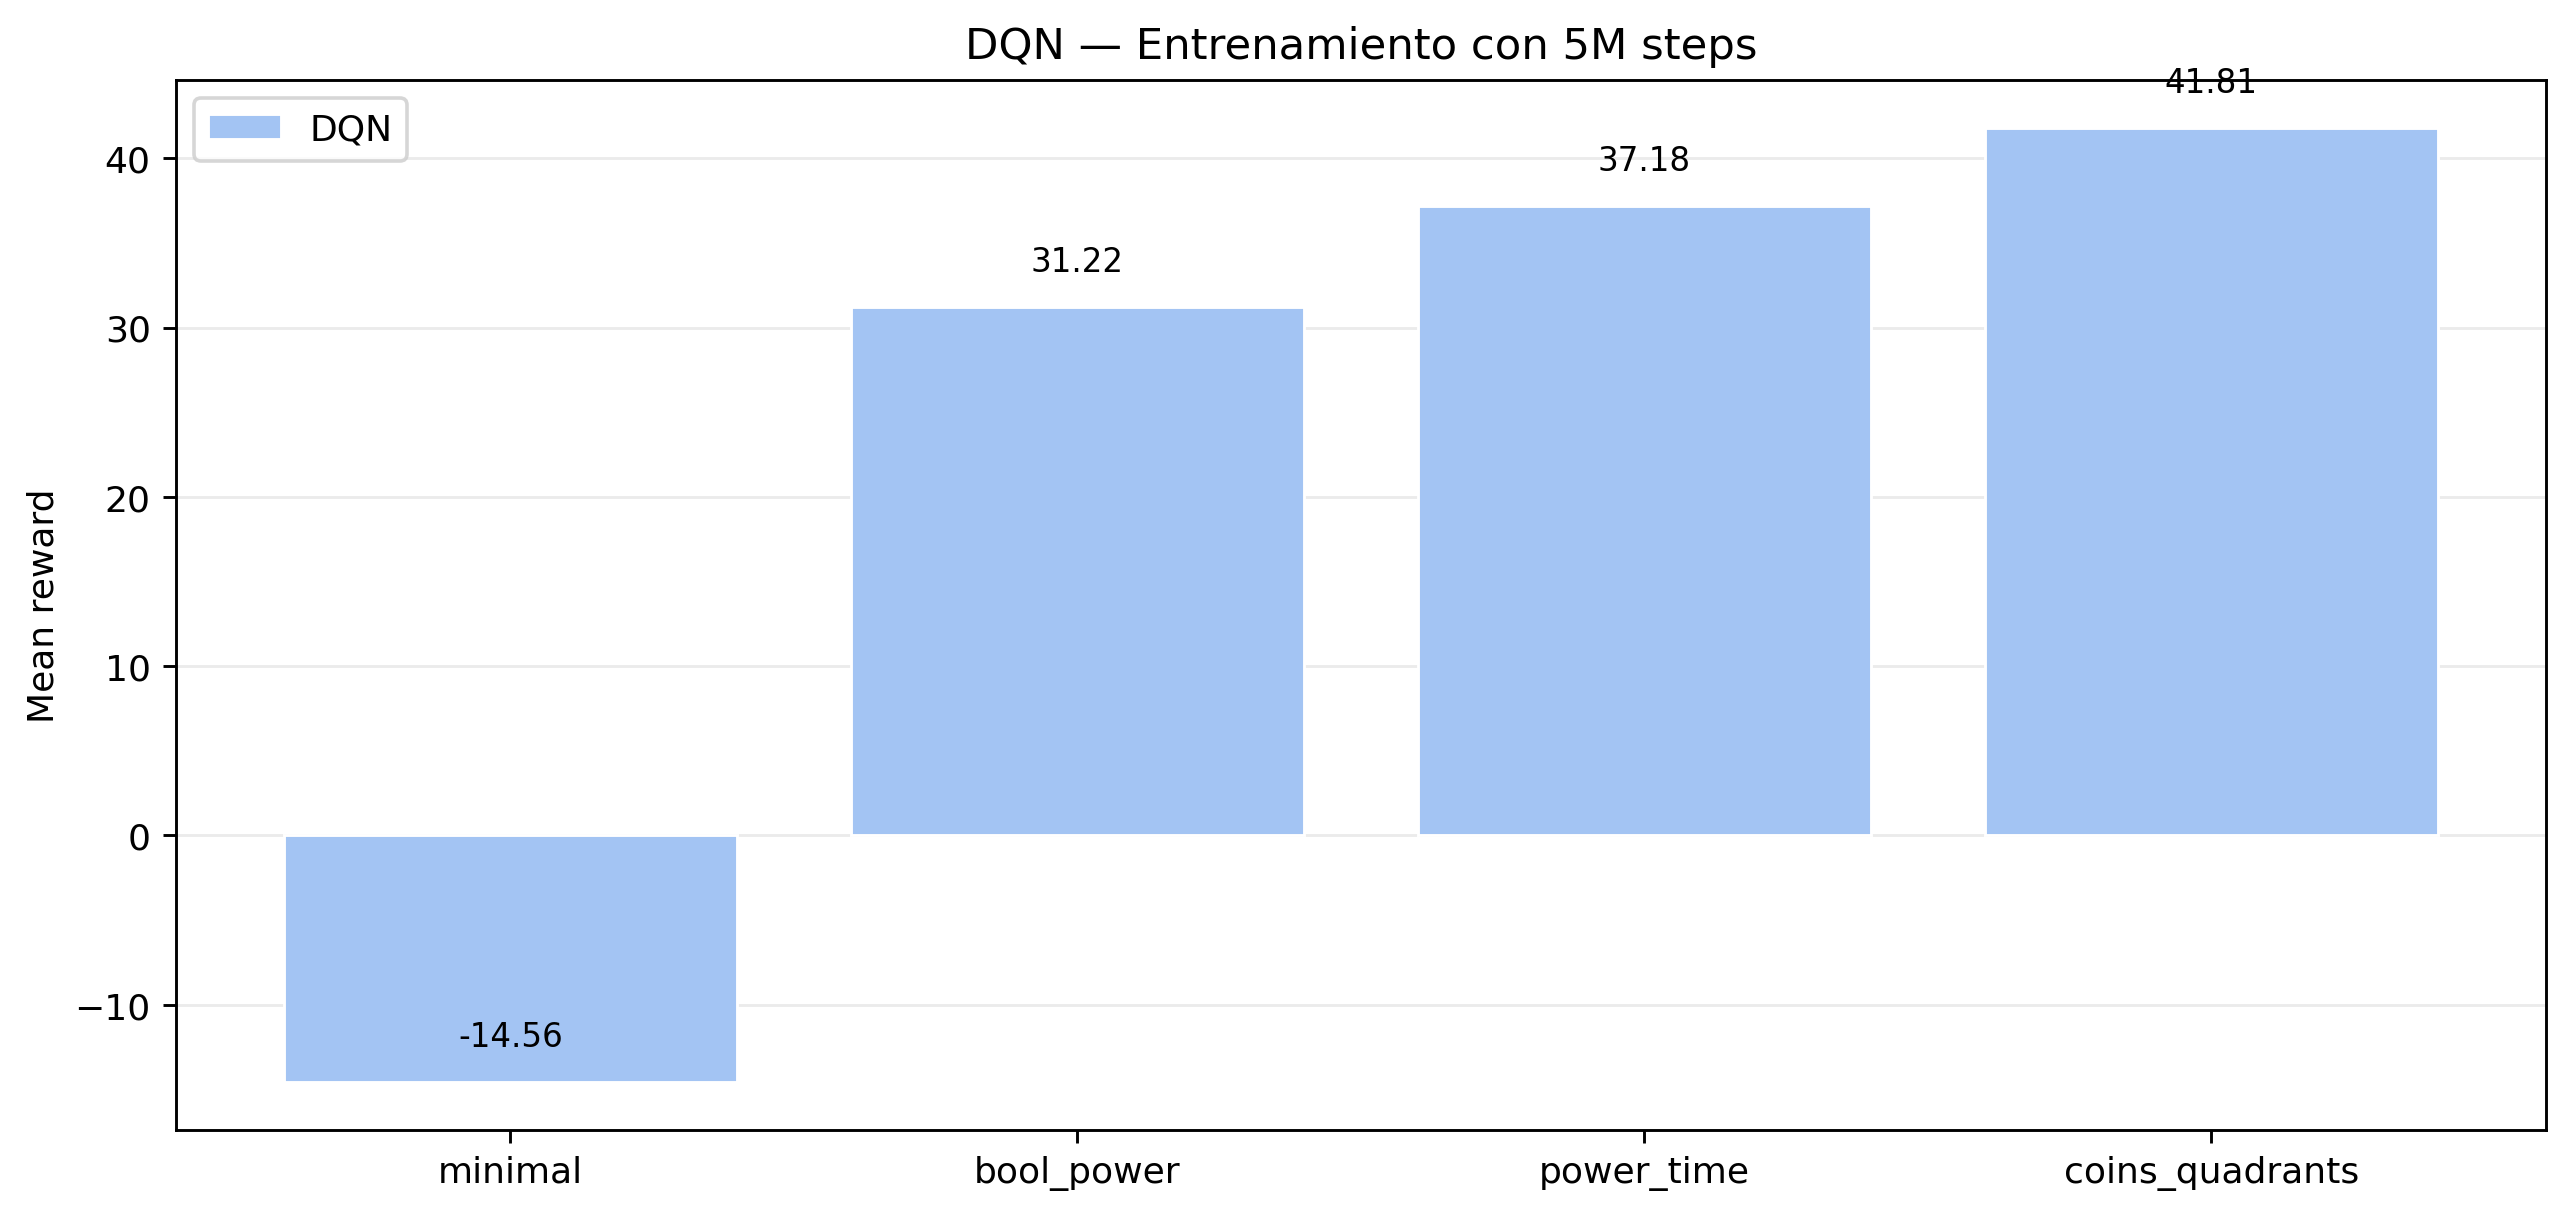
\includegraphics[width=0.5\textwidth]{./figs/graphics/dqn_mean_reward.png}
\caption{Mean reward con algoritmo de DQN entrenado con 5M de steps}
\label{fig:mean_reward_dqn}
\end{figure}

No obstante, a pesar de estas mejoras en la recompensa acumulada, DQN no consigue completar el entorno de forma consistente en ninguno de los modos de observación analizados. La tasa de éxito es nula en todos los casos, y no se observan episodios cercanos a la resolución completa del nivel. Este comportamiento se refleja también en el \textit{completion ratio}, que alcanza su valor máximo en el modo \textit{coins\_quadrants} (0.68), seguido por \textit{power\_time} (0.61) y \textit{bool\_power} (0.53). El modo de observación mínima presenta el menor ratio de completado (0.47), lo que refuerza la idea de que la falta de información espacial limita la capacidad del agente para cubrir el entorno de manera efectiva. En todos los casos, la tasa de éxito permanece nula, lo que indica que el agente no logra completar el nivel de forma consistente.

\begin{figure}[h]
\centering
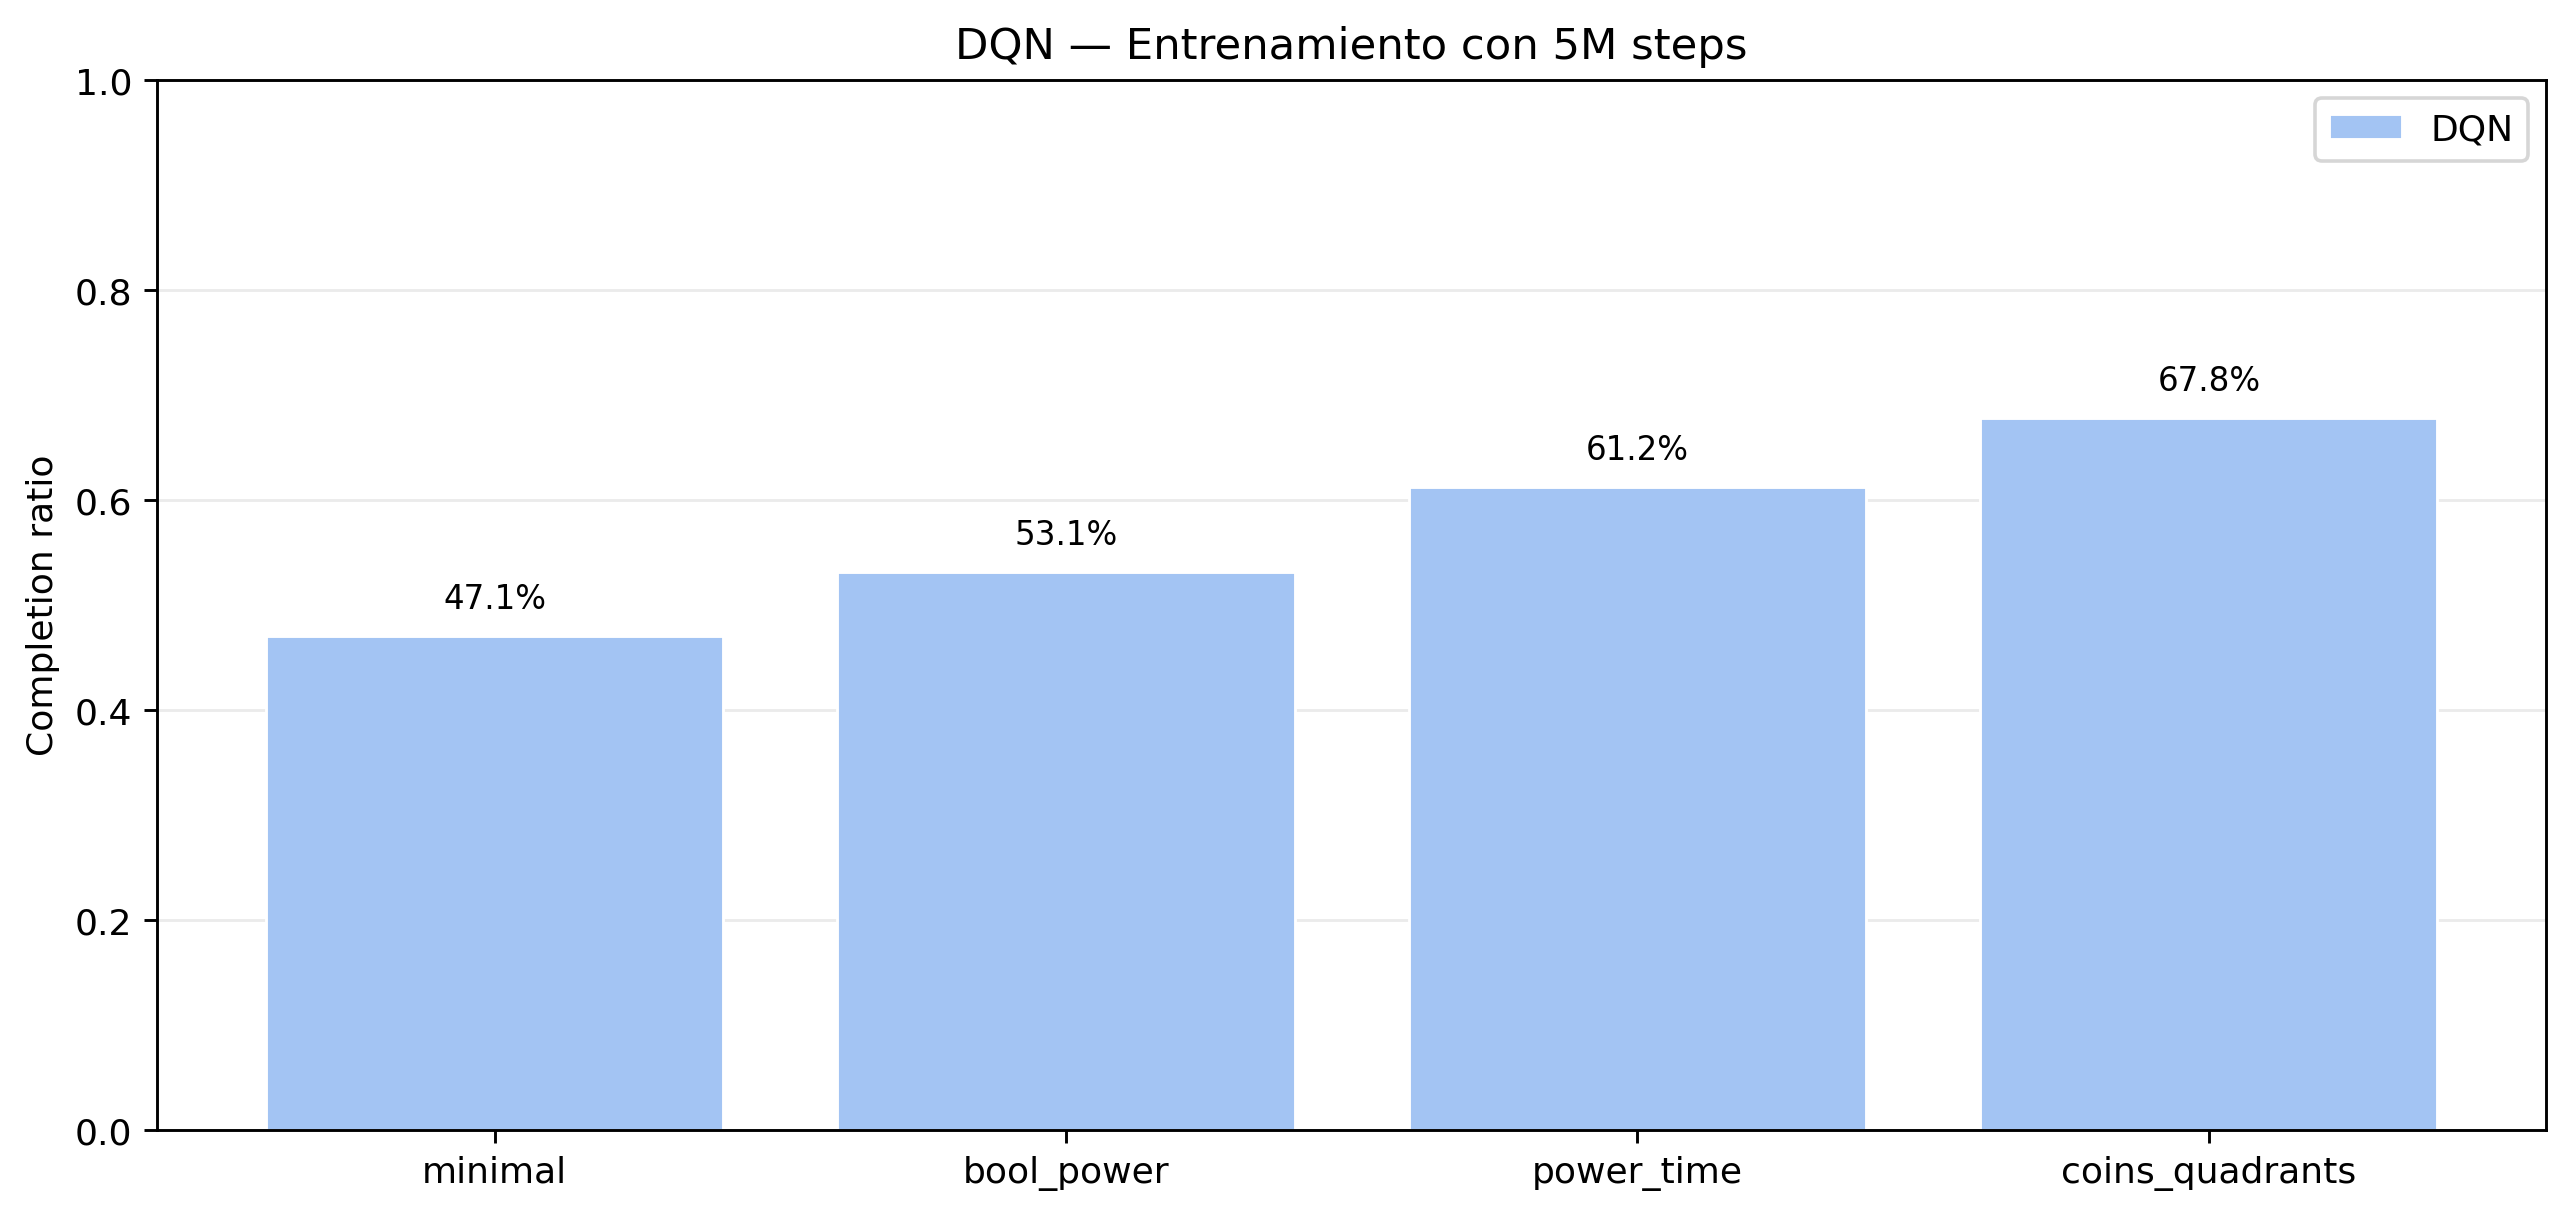
\includegraphics[width=0.5\textwidth]{./figs/graphics/dqn_completion_ratio.png}
\caption{Completion ratio con algoritmo de DQN entrenado con 5M de steps}
\label{fig:completion_ratio_dqn}
\end{figure}

En términos de estabilidad, los resultados evidencian una elevada variabilidad en el rendimiento entre episodios, reflejada en desviaciones estándar de la recompensa relativamente altas, especialmente en los modos con observaciones más complejas. Asimismo, la duración media de los episodios es considerablemente elevada, lo que sugiere comportamientos poco eficientes y trayectorias prolongadas que no conducen de forma sistemática a la finalización exitosa del episodio.

\begin{figure}[h]
\centering
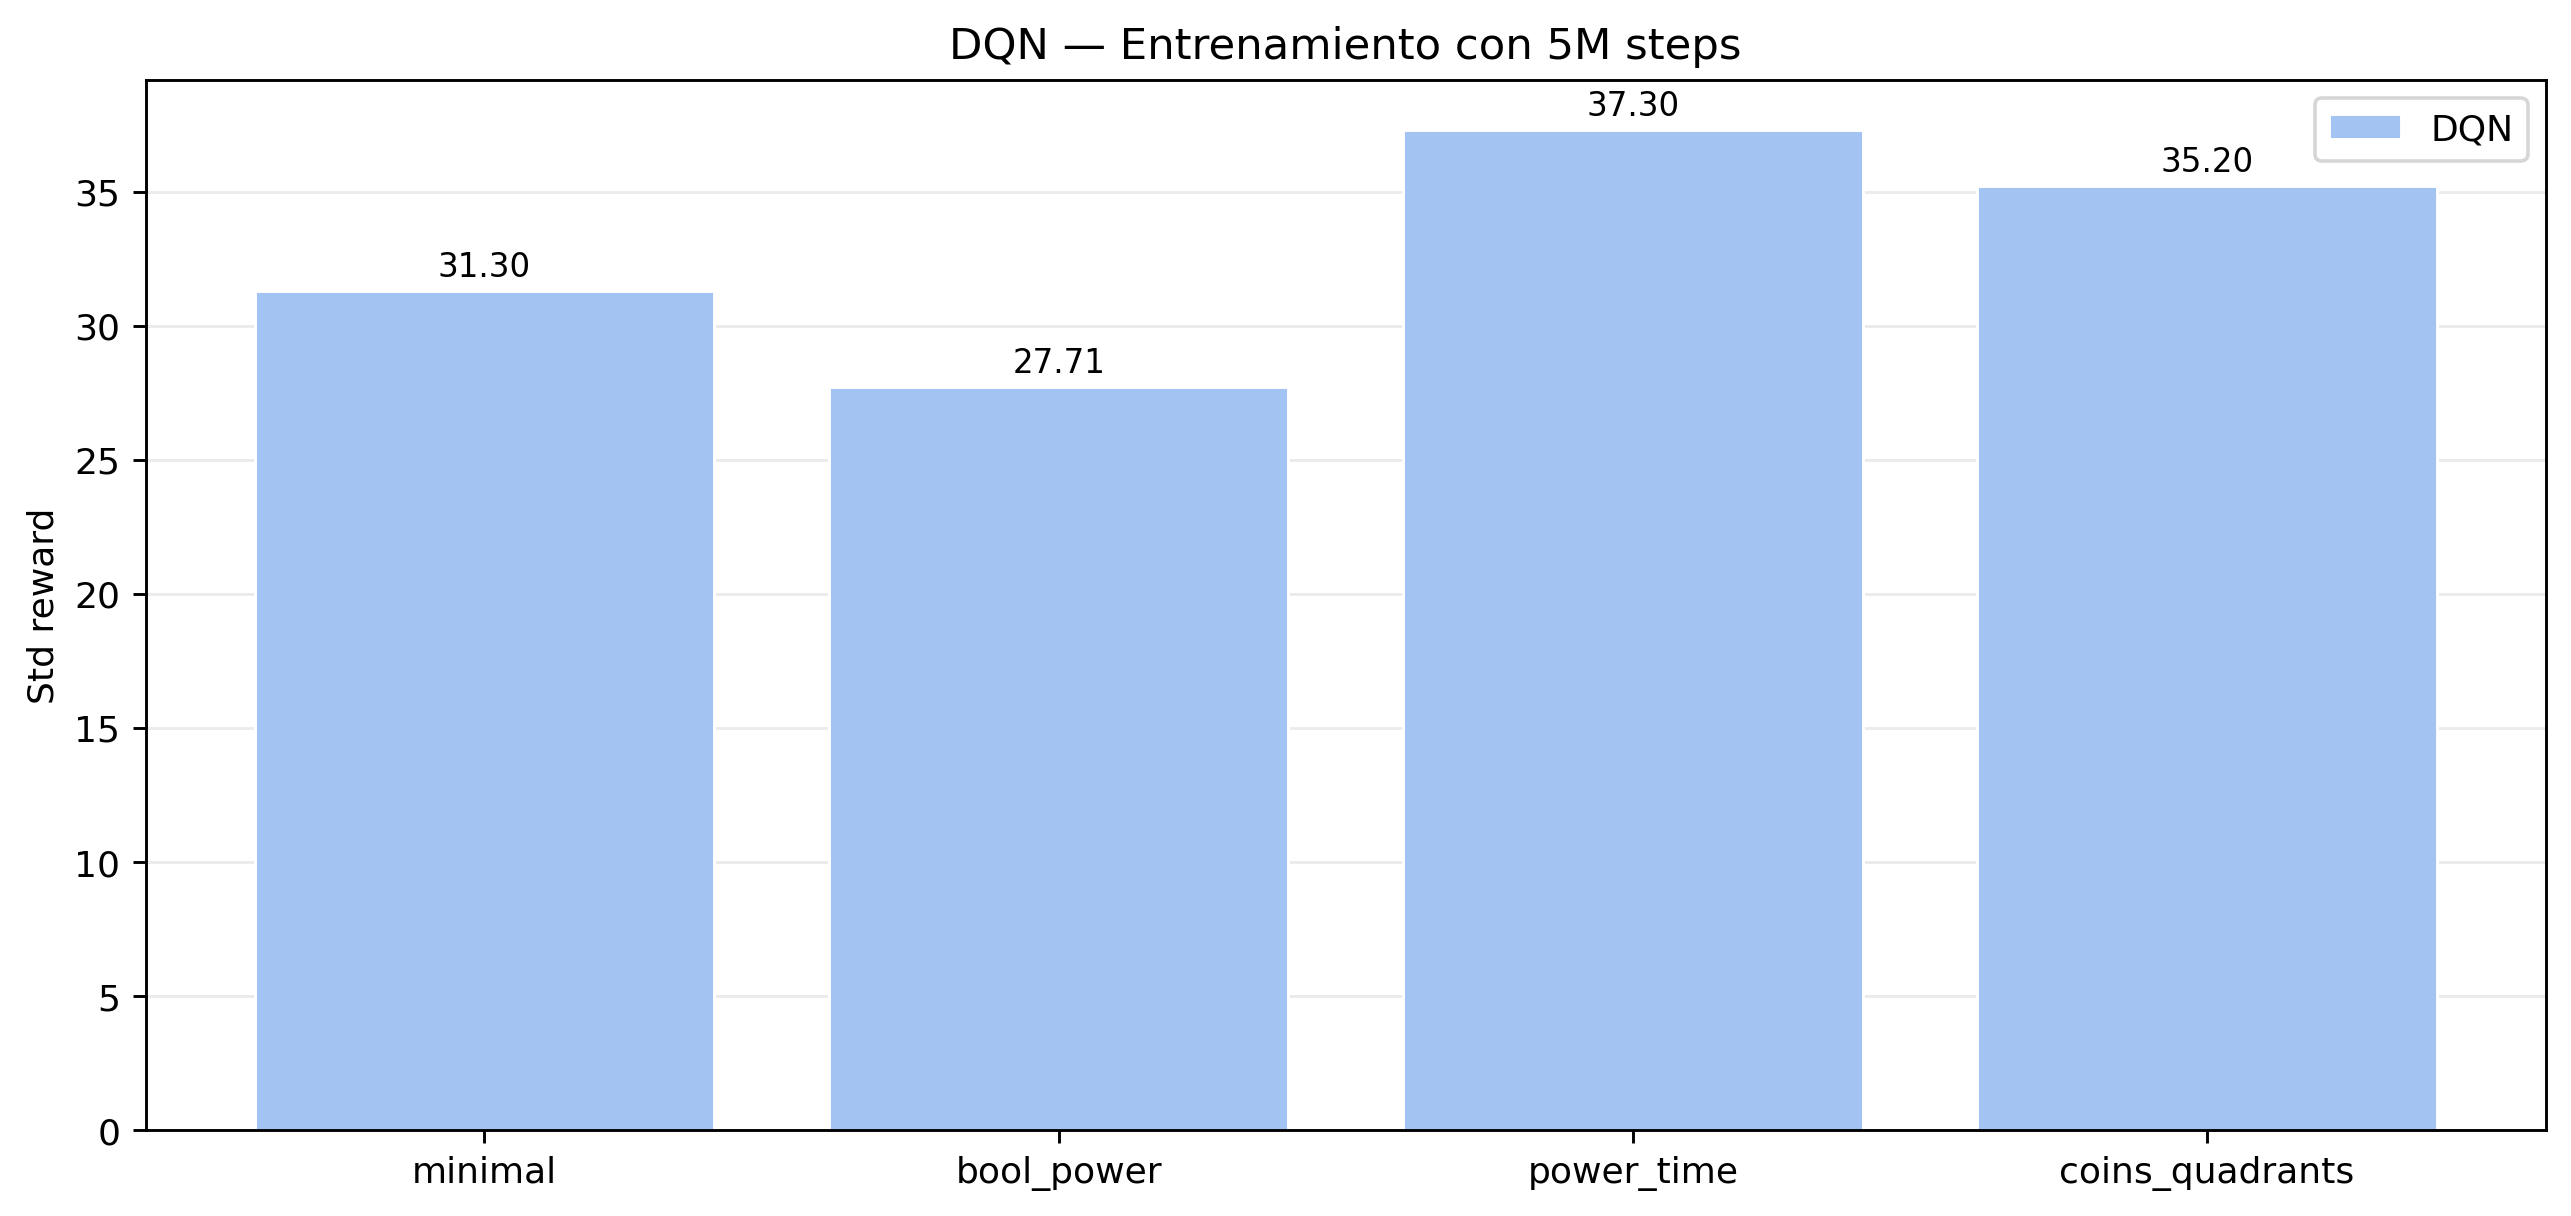
\includegraphics[width=0.5\textwidth]{./figs/graphics/dqn_std_reward.png}
\caption{Std reward con algoritmo de DQN entrenado con 5M de steps}
\label{fig:std_reward_dqn}
\end{figure}

El análisis de los distintos modos de observación indica que, en el caso de DQN, el aumento de la complejidad del estado se traduce en una mejora progresiva del rendimiento, tanto en términos de recompensa media como de \textit{completion ratio}. A medida que se incorporan observaciones más informativas, el agente es capaz de explotar mejor la estructura del entorno y cubrir una mayor fracción del mapa. No obstante, esta mejora no se refleja en una tasa de éxito no nula, lo que pone de manifiesto que, pese al mayor progreso parcial, el agente no logra resolver la tarea de forma consistente.

Finalmente, cabe destacar el elevado coste computacional asociado al entrenamiento de DQN. El número de pasos necesarios para alcanzar un comportamiento razonablemente estable, junto con la necesidad de múltiples ejecuciones para el ajuste de hiperparámetros, limita la viabilidad de realizar estudios exhaustivos con este algoritmo en comparación con métodos actor-crítico más eficientes.

En conjunto, estos resultados posicionan a DQN como un algoritmo capaz de aprender comportamientos parciales en el entorno \textit{SimplePacmanEnv}, pero con limitaciones claras en términos de estabilidad, eficiencia y capacidad de resolución completa de la tarea.

\subsection{Resultados con Advantage Actor-Critic (A2C)}

En este apartado se presentan los resultados obtenidos con el algoritmo Advantage Actor-Critic (A2C) bajo las distintas configuraciones de observación definidas en el entorno \textit{SimplePacmanEnv}. A diferencia de DQN, A2C permitió realizar un mayor número de ejecuciones exhaustivas debido a su menor coste computacional, lo que facilitó un análisis más detallado del impacto de los hiperparámetros y de la complejidad del estado.

Se evaluaron tres configuraciones principales de entrenamiento, correspondientes a diferentes niveles de optimización de hiperparámetros mediante Optuna: (i) 40 \textit{trials} con 300\,000 pasos por prueba, (ii) 40 \textit{trials} con 1 millón de pasos y (iii) 200 \textit{trials} con 1 millón de pasos. En todos los casos, los modelos resultantes fueron entrenados durante 5 millones de pasos y evaluados posteriormente sobre 100 episodios independientes.

Los resultados muestran que A2C es capaz de aprender políticas estables y consistentes en todas las configuraciones de observación analizadas. En comparación con DQN, el algoritmo presenta una menor variabilidad en la recompensa entre episodios y una duración media de los episodios significativamente más reducida, lo que indica un comportamiento más estructurado y menos errático. No obstante, al igual que en el caso de DQN, A2C no logra completar el entorno de forma exitosa en ninguno de los modos de observación evaluados, con tasas de éxito y episodios cercanos a la resolución completas nulas.

El análisis de la complejidad del estado revela diferencias claras entre los distintos modos de observación. Las configuraciones que incorporan información contextual adicional, como el temporizador del comodín (\textit{power\_time}), presentan de forma consistente mayores ratios de completado parcial del entorno, alcanzando valores cercanos al 18\%. Por el contrario, el modo de observación mínima obtiene los peores resultados, con ratios de completado notablemente inferiores, lo que sugiere que una representación excesivamente simple limita la capacidad del agente para desarrollar estrategias efectivas.

\begin{figure}[h]
\centering
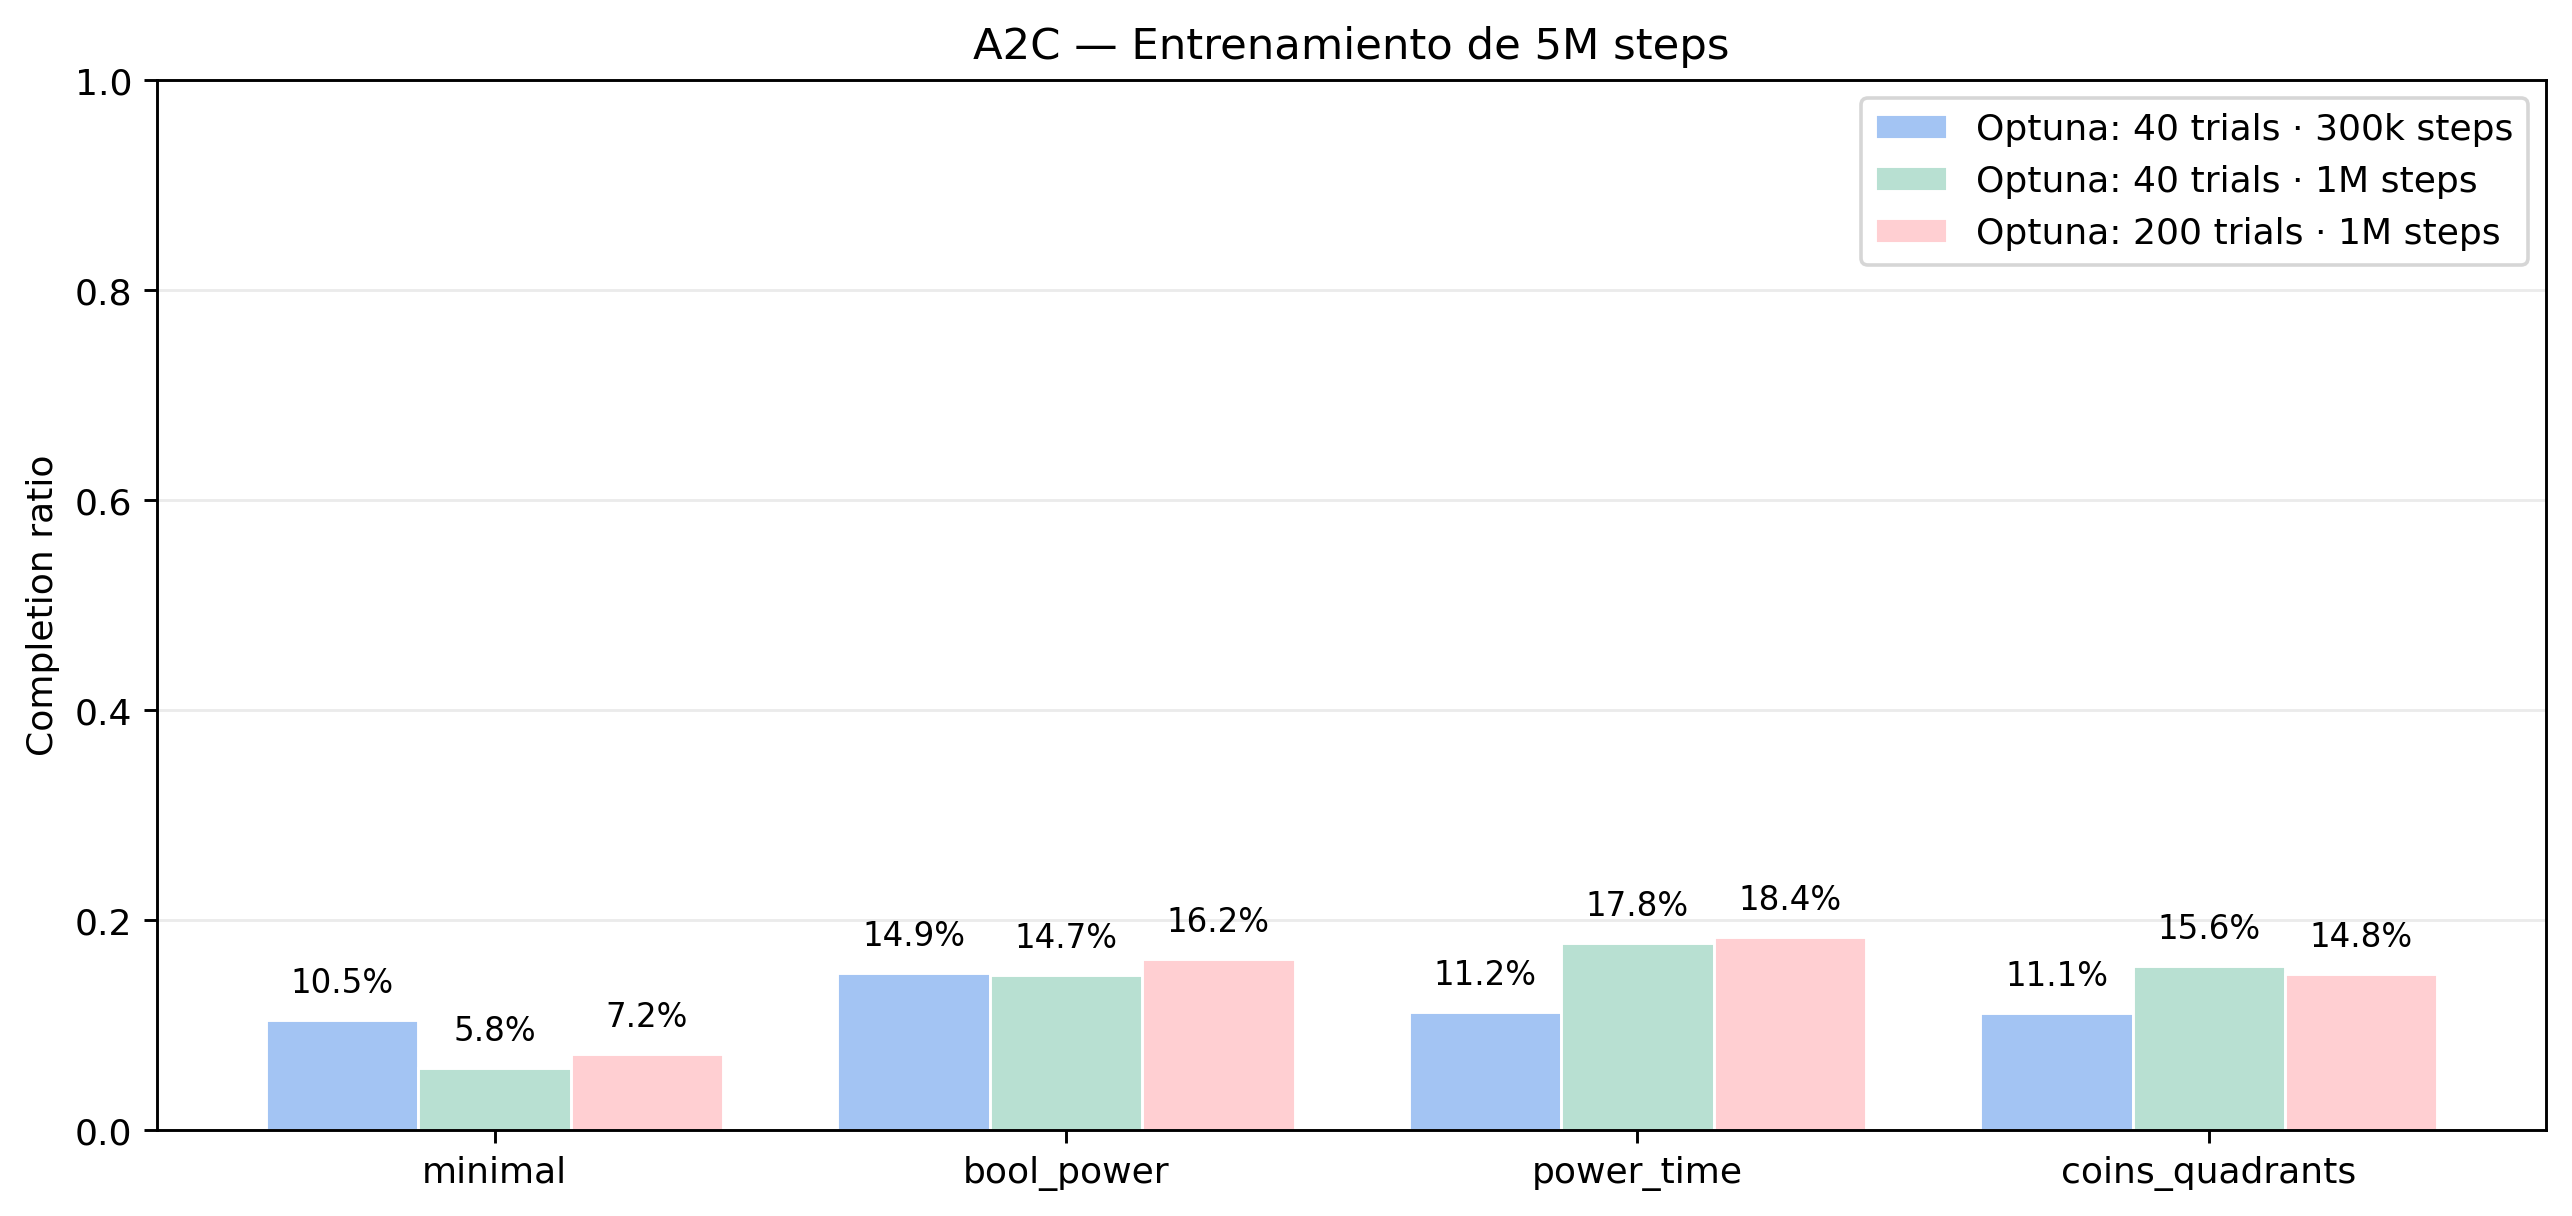
\includegraphics[width=0.5\textwidth]{./figs/graphics/a2c_optuna_completion_ratio.png}
\caption{Completion ratio con algoritmo de A2C entrenado con 5M de steps}
\label{fig:completion_ratio_a2c}
\end{figure}

En cuanto al impacto de la optimización de hiperparámetros, los resultados indican que el aumento del esfuerzo computacional no se traduce necesariamente en mejoras sustanciales del rendimiento. Las configuraciones más exhaustivas, con un mayor número de \textit{trials} y pasos de entrenamiento, no presentan diferencias significativas respecto a configuraciones más ligeras, lo que apunta a un fenómeno de rendimientos decrecientes en el proceso de ajuste de A2C para este entorno.

\begin{figure}[h]
\centering
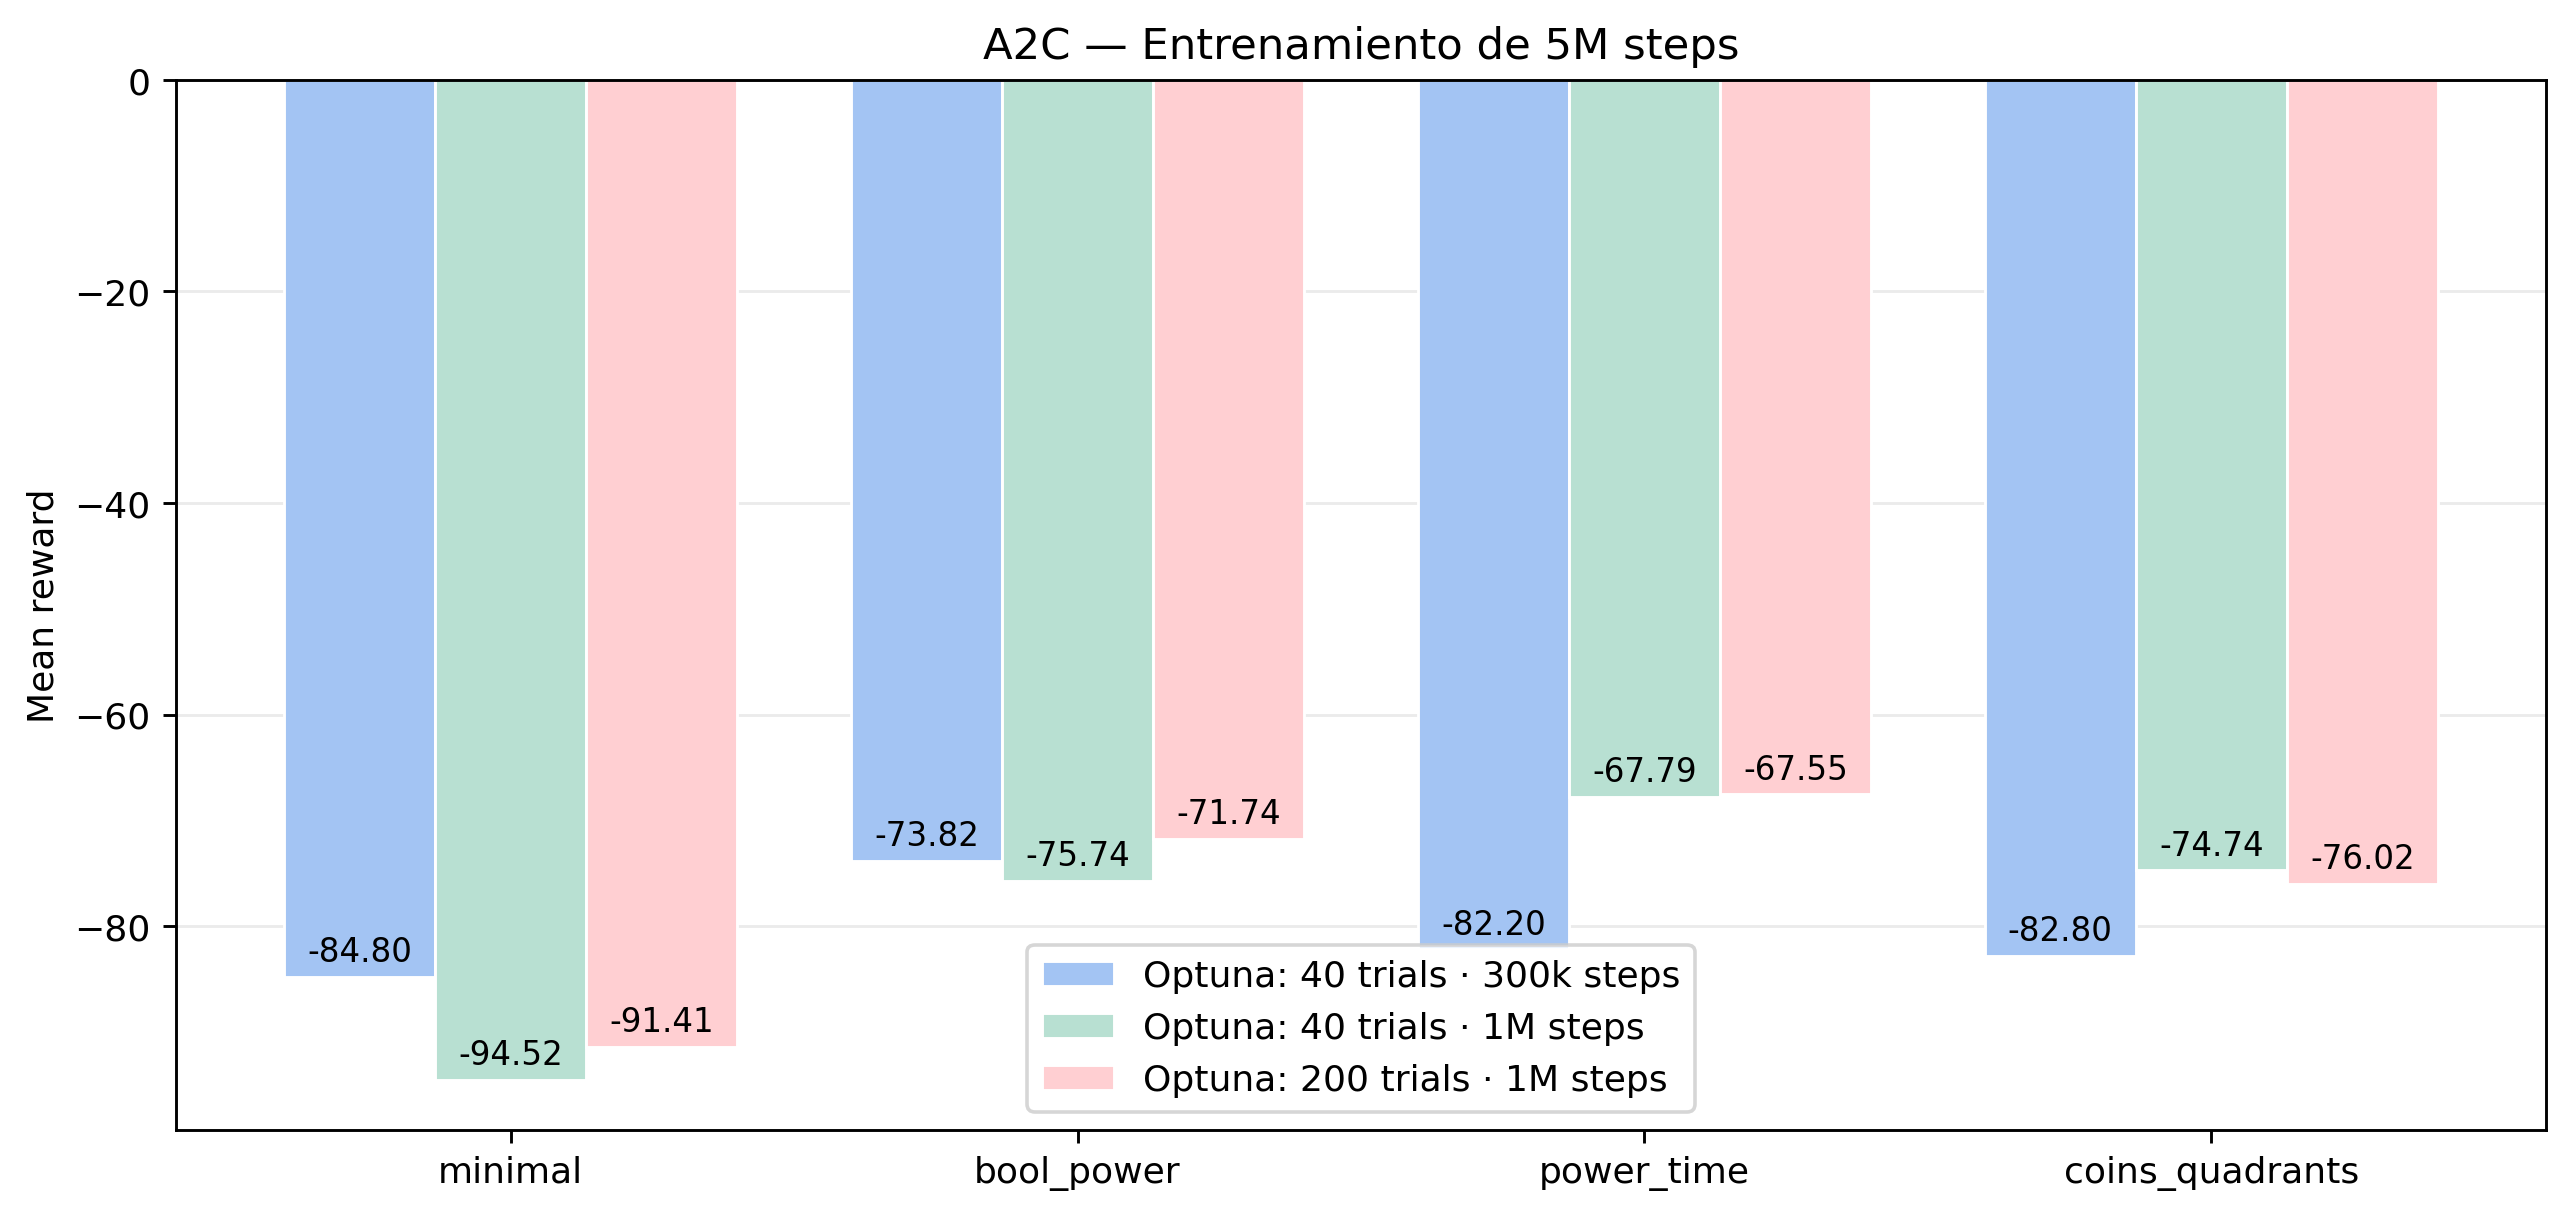
\includegraphics[width=0.5\textwidth]{./figs/graphics/a2c_optuna_mean_reward.png}
\caption{Completion ratio con algoritmo de A2C entrenado con 5M de steps}
\label{fig:mean_reward_a2c}
\end{figure}

\begin{figure}[h]
\centering
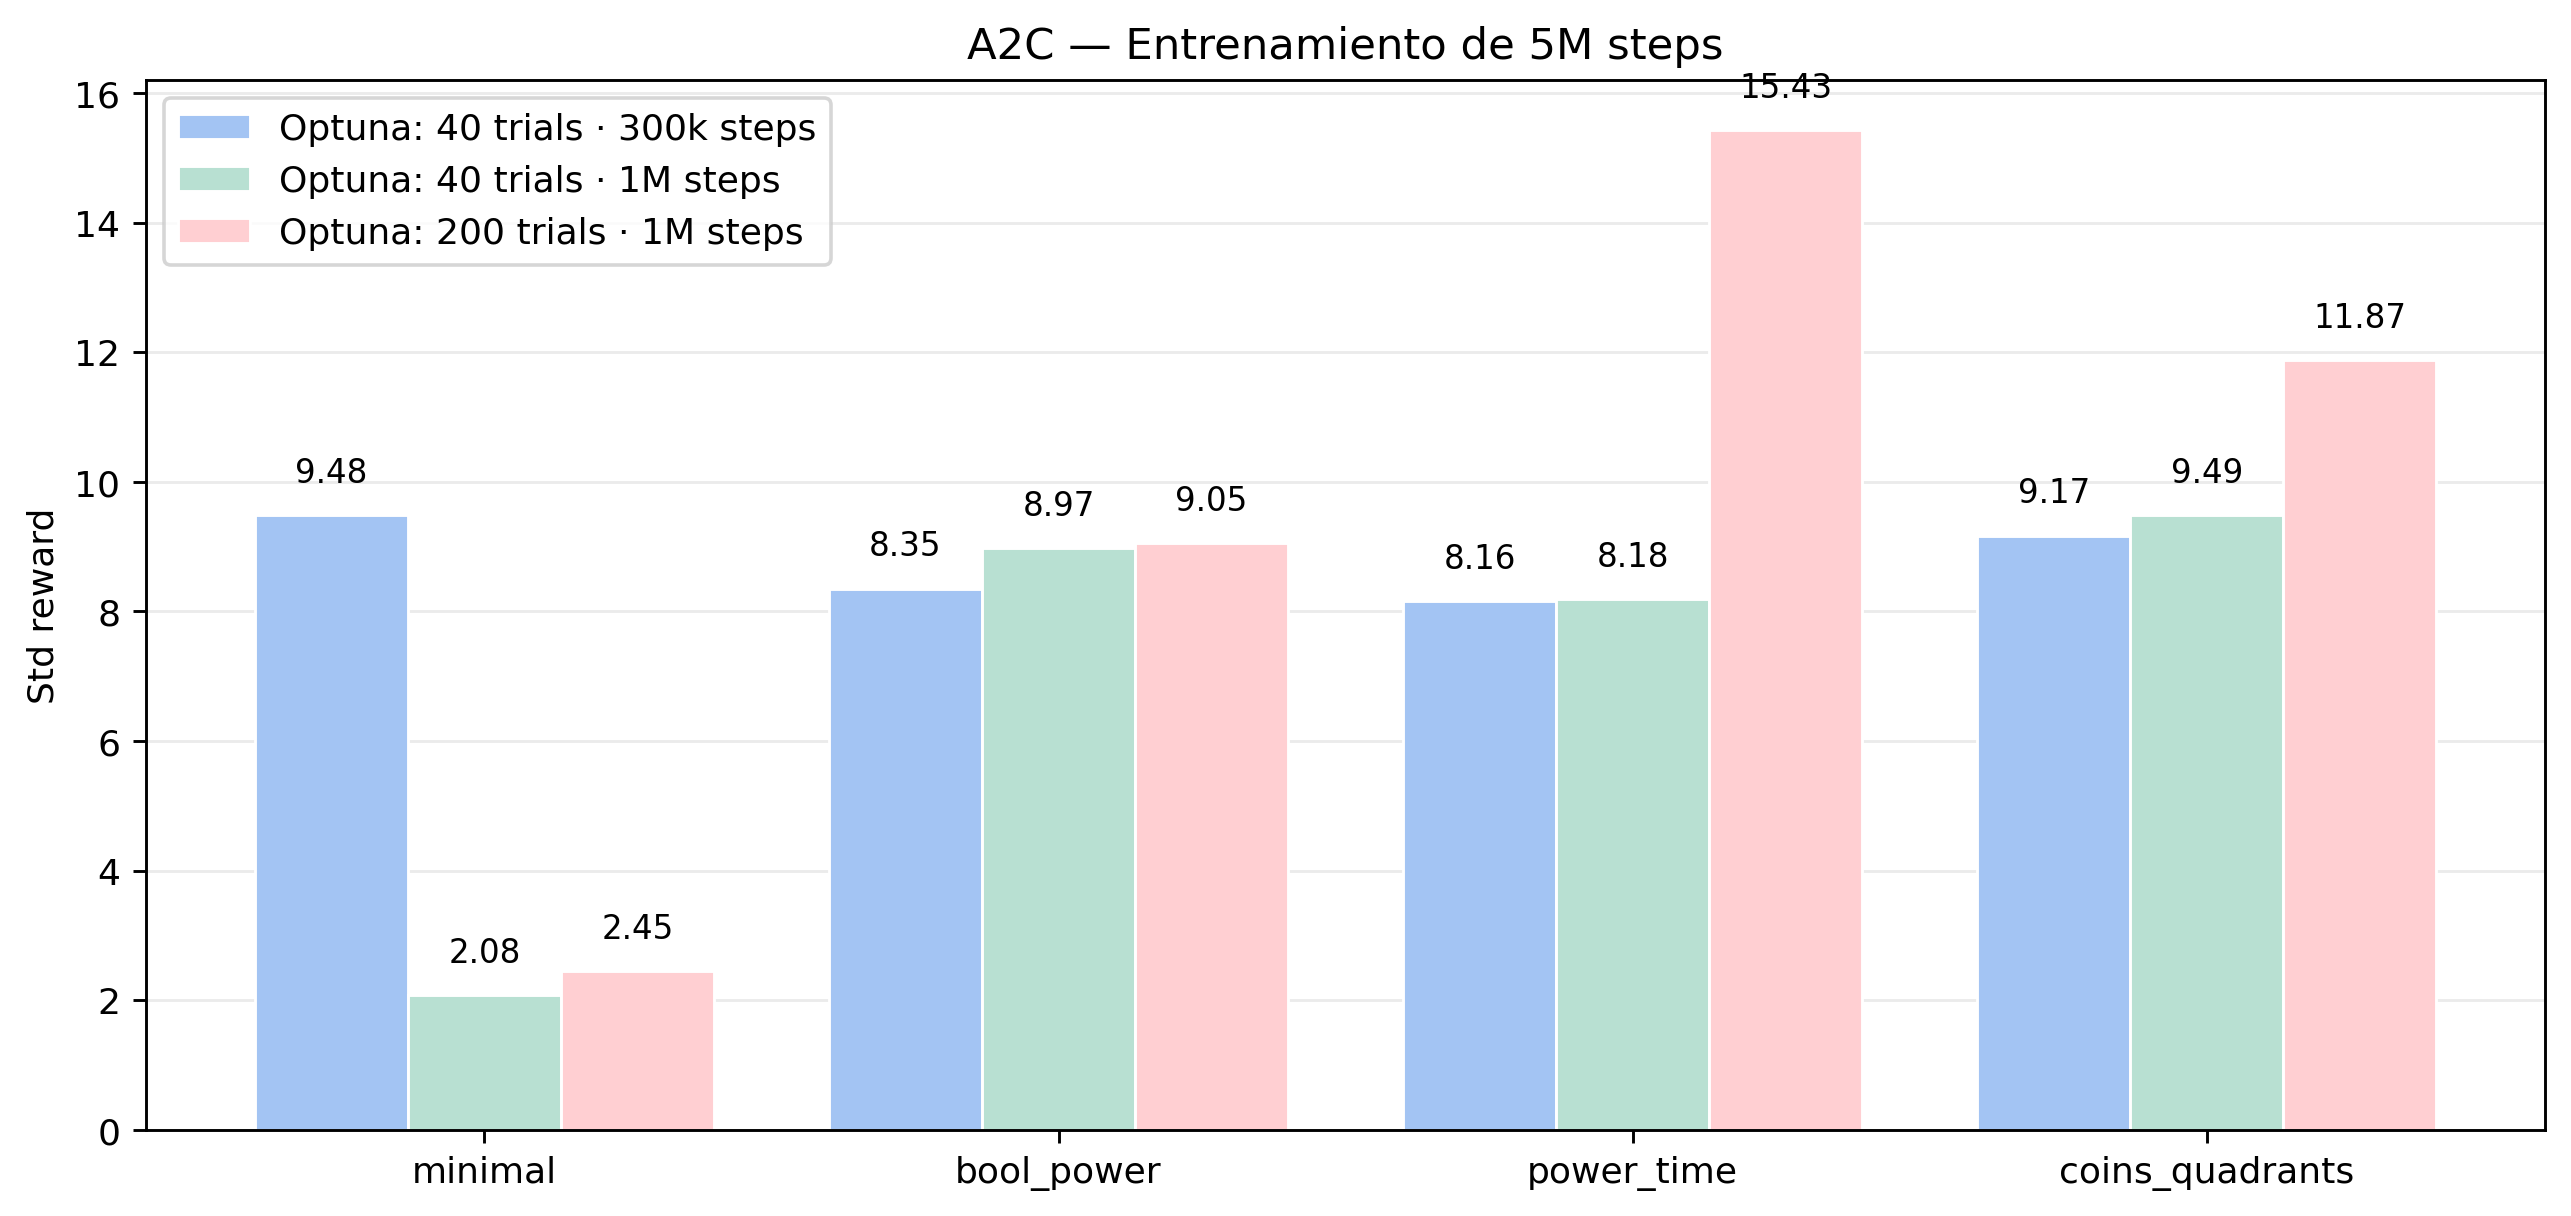
\includegraphics[width=0.5\textwidth]{./figs/graphics/a2c_optuna_std_reward.png}
\caption{Std reward con algoritmo de A2C entrenado con 5M de steps}
\label{fig:std_reward_a2c}
\end{figure}

En conjunto, estos resultados muestran que A2C ofrece una mayor estabilidad que DQN y se beneficia de observaciones más informativas, pero sigue mostrando limitaciones claras para resolver completamente la tarea. Este comportamiento refuerza la idea de que la complejidad del estado, si bien necesaria para aprender políticas útiles, no garantiza por sí sola el éxito del aprendizaje en entornos con dinámicas adversas.

\subsection{Resultados con Proximal Policy Optimization (PPO)}

En este apartado se presentan los resultados obtenidos con el algoritmo Proximal Policy Optimization (PPO) bajo las distintas configuraciones de observación del entorno \textit{SimplePacmanEnv}. PPO se ha evaluado utilizando dos niveles de optimización de hiperparámetros mediante Optuna, correspondientes a una configuración ligera (40 \textit{trials} con 300\,000 pasos por prueba) y una configuración exhaustiva (200 \textit{trials} con 1 millón de pasos por prueba). En ambos casos, los modelos seleccionados se entrenaron posteriormente durante 5 millones de pasos antes de su evaluación final.

Los resultados evidencian una marcada sensibilidad de PPO al grado de optimización de hiperparámetros. Las configuraciones menos exhaustivas presentan un rendimiento limitado, con recompensas medias negativas y bajos ratios de completado parcial del entorno. En contraste, los modelos entrenados a partir de una optimización más exhaustiva muestran una mejora sustancial en todas las métricas consideradas, lo que pone de manifiesto la importancia del ajuste fino de los parámetros en este algoritmo.

Bajo la configuración más exhaustiva, PPO obtiene resultados competitivos, especialmente en configuraciones de observación más simples, como el modo \textit{minimal}. Sin embargo, en modos de observación más ricos, DQN alcanza valores superiores tanto de recompensa media como de \textit{completion ratio}. Estos resultados indican que, si bien PPO es capaz de aprender políticas efectivas cuando se dispone de una optimización adecuada, no domina de forma sistemática frente a DQN en este entorno.

\begin{figure}[h]
\centering
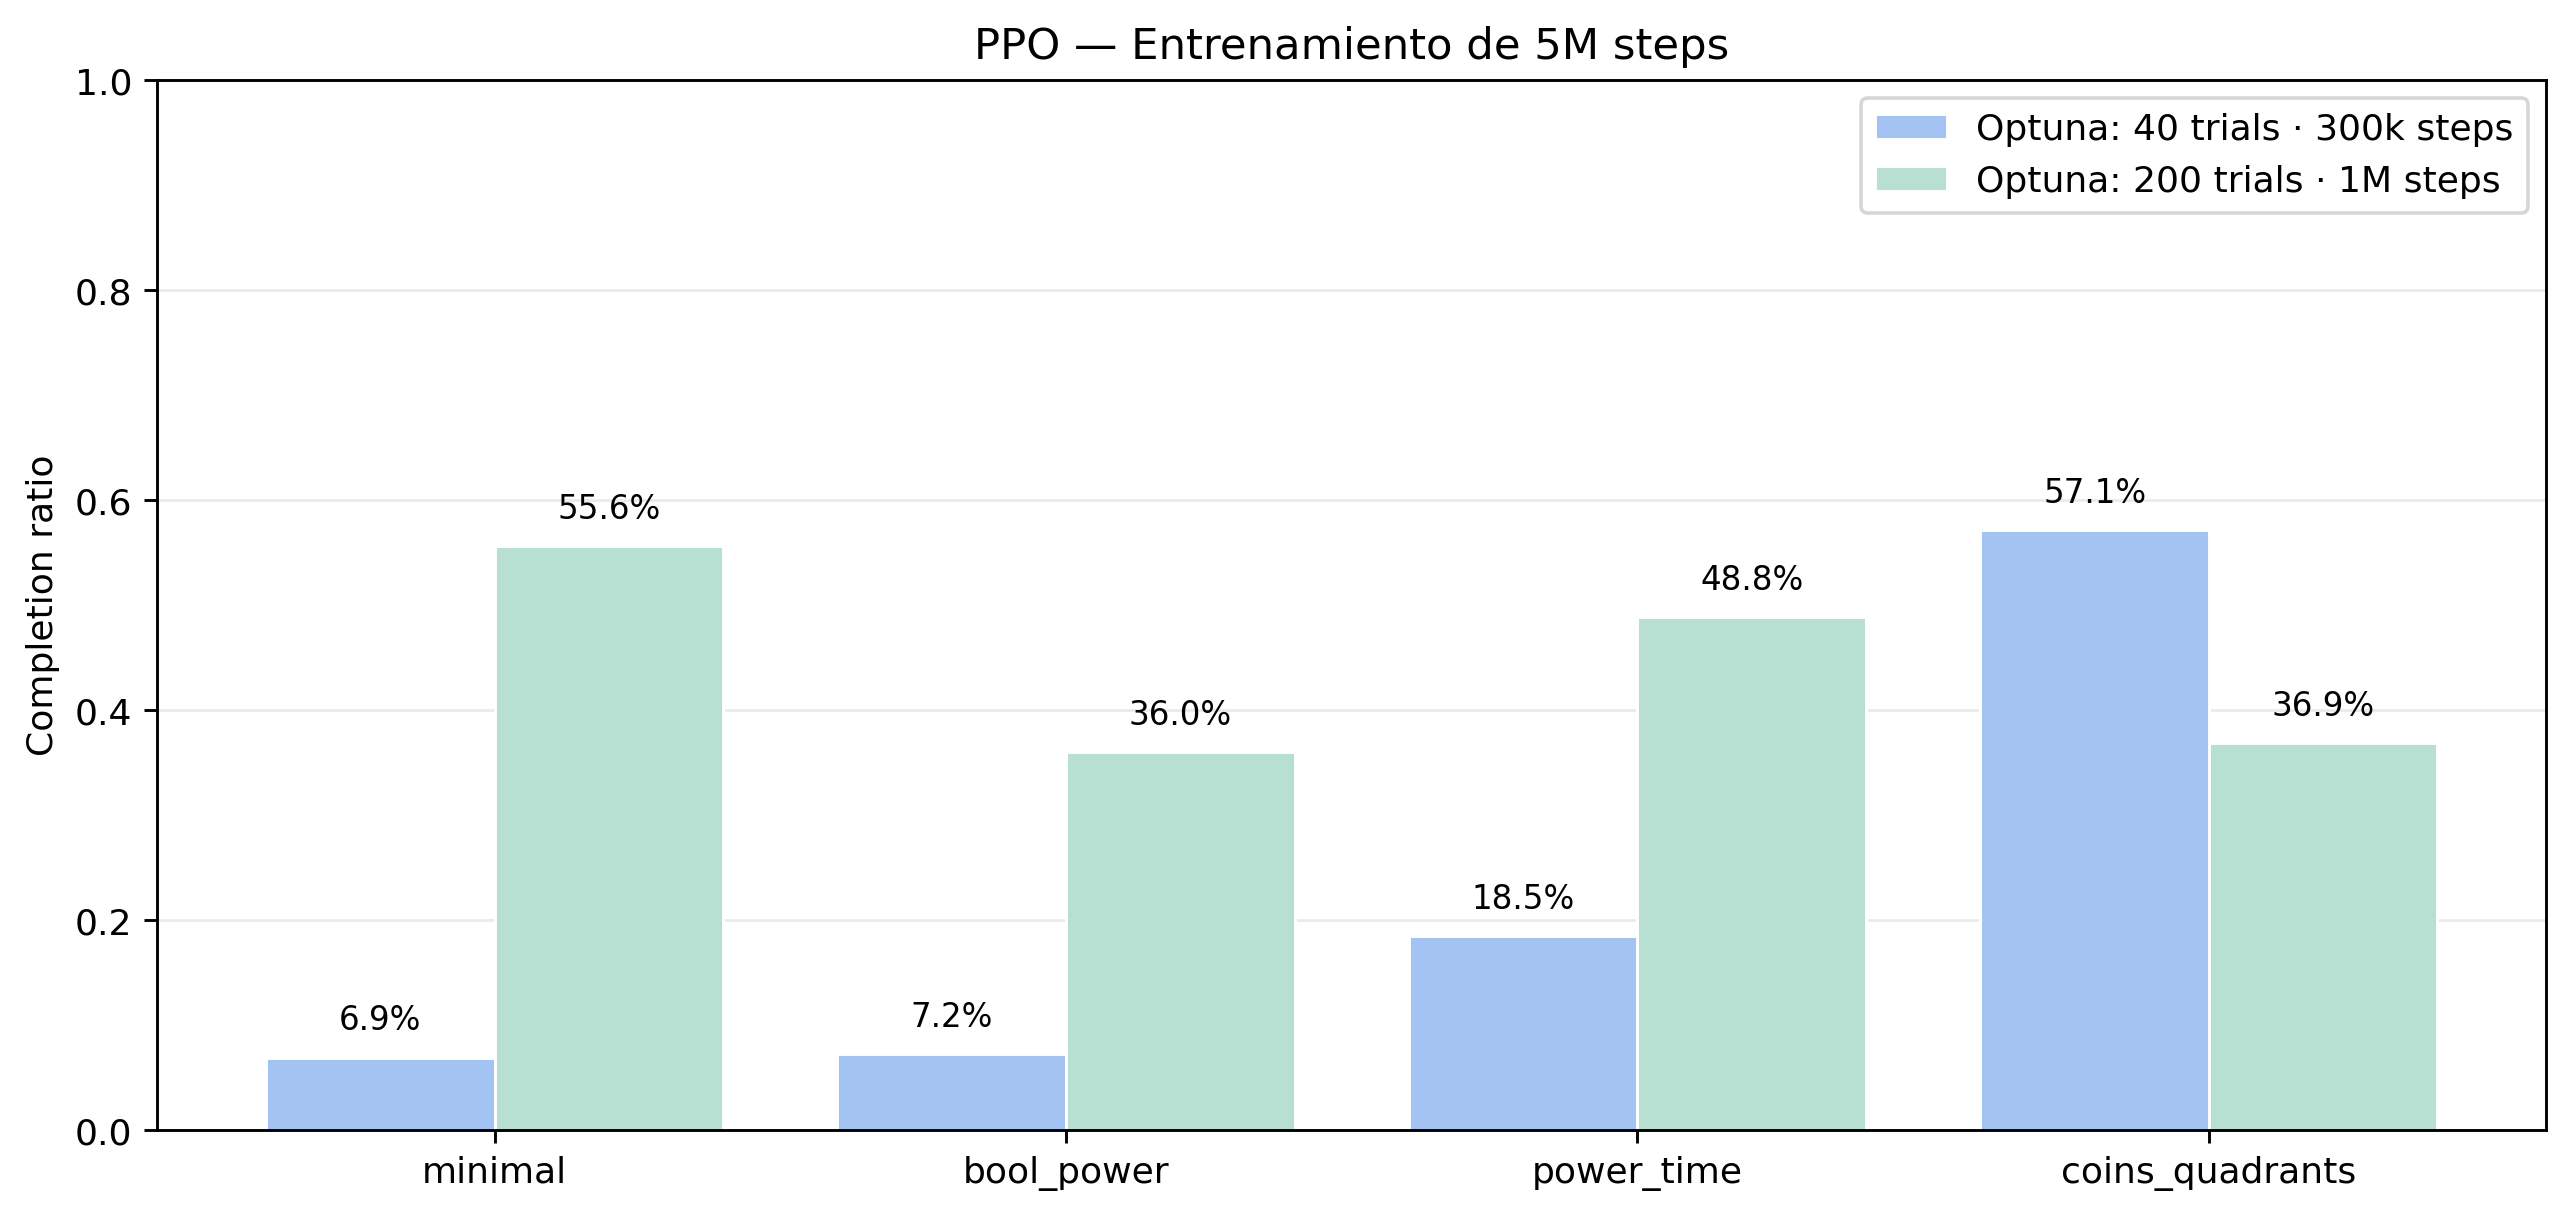
\includegraphics[width=0.5\textwidth]{./figs/graphics/ppo_optuna_completion_ratio.png}
\caption{Completion ratio con algoritmo de PPO entrenado con 5M de steps}
\label{fig:std_reward_a2c}
\end{figure}

No obstante, a pesar de estas mejoras, PPO no logra resolver completamente el entorno en ninguno de los modos de observación evaluados, manteniendo tasas de éxito nulas en todas las configuraciones. Asimismo, se observa una elevada variabilidad en la recompensa entre episodios y una duración media de los episodios considerablemente elevada, especialmente en los modelos mejor optimizados. Este comportamiento indica que, si bien las políticas aprendidas son más ambiciosas y exploratorias, aún carecen de la consistencia necesaria para completar la tarea de forma fiable.

\begin{figure}[h]
\centering
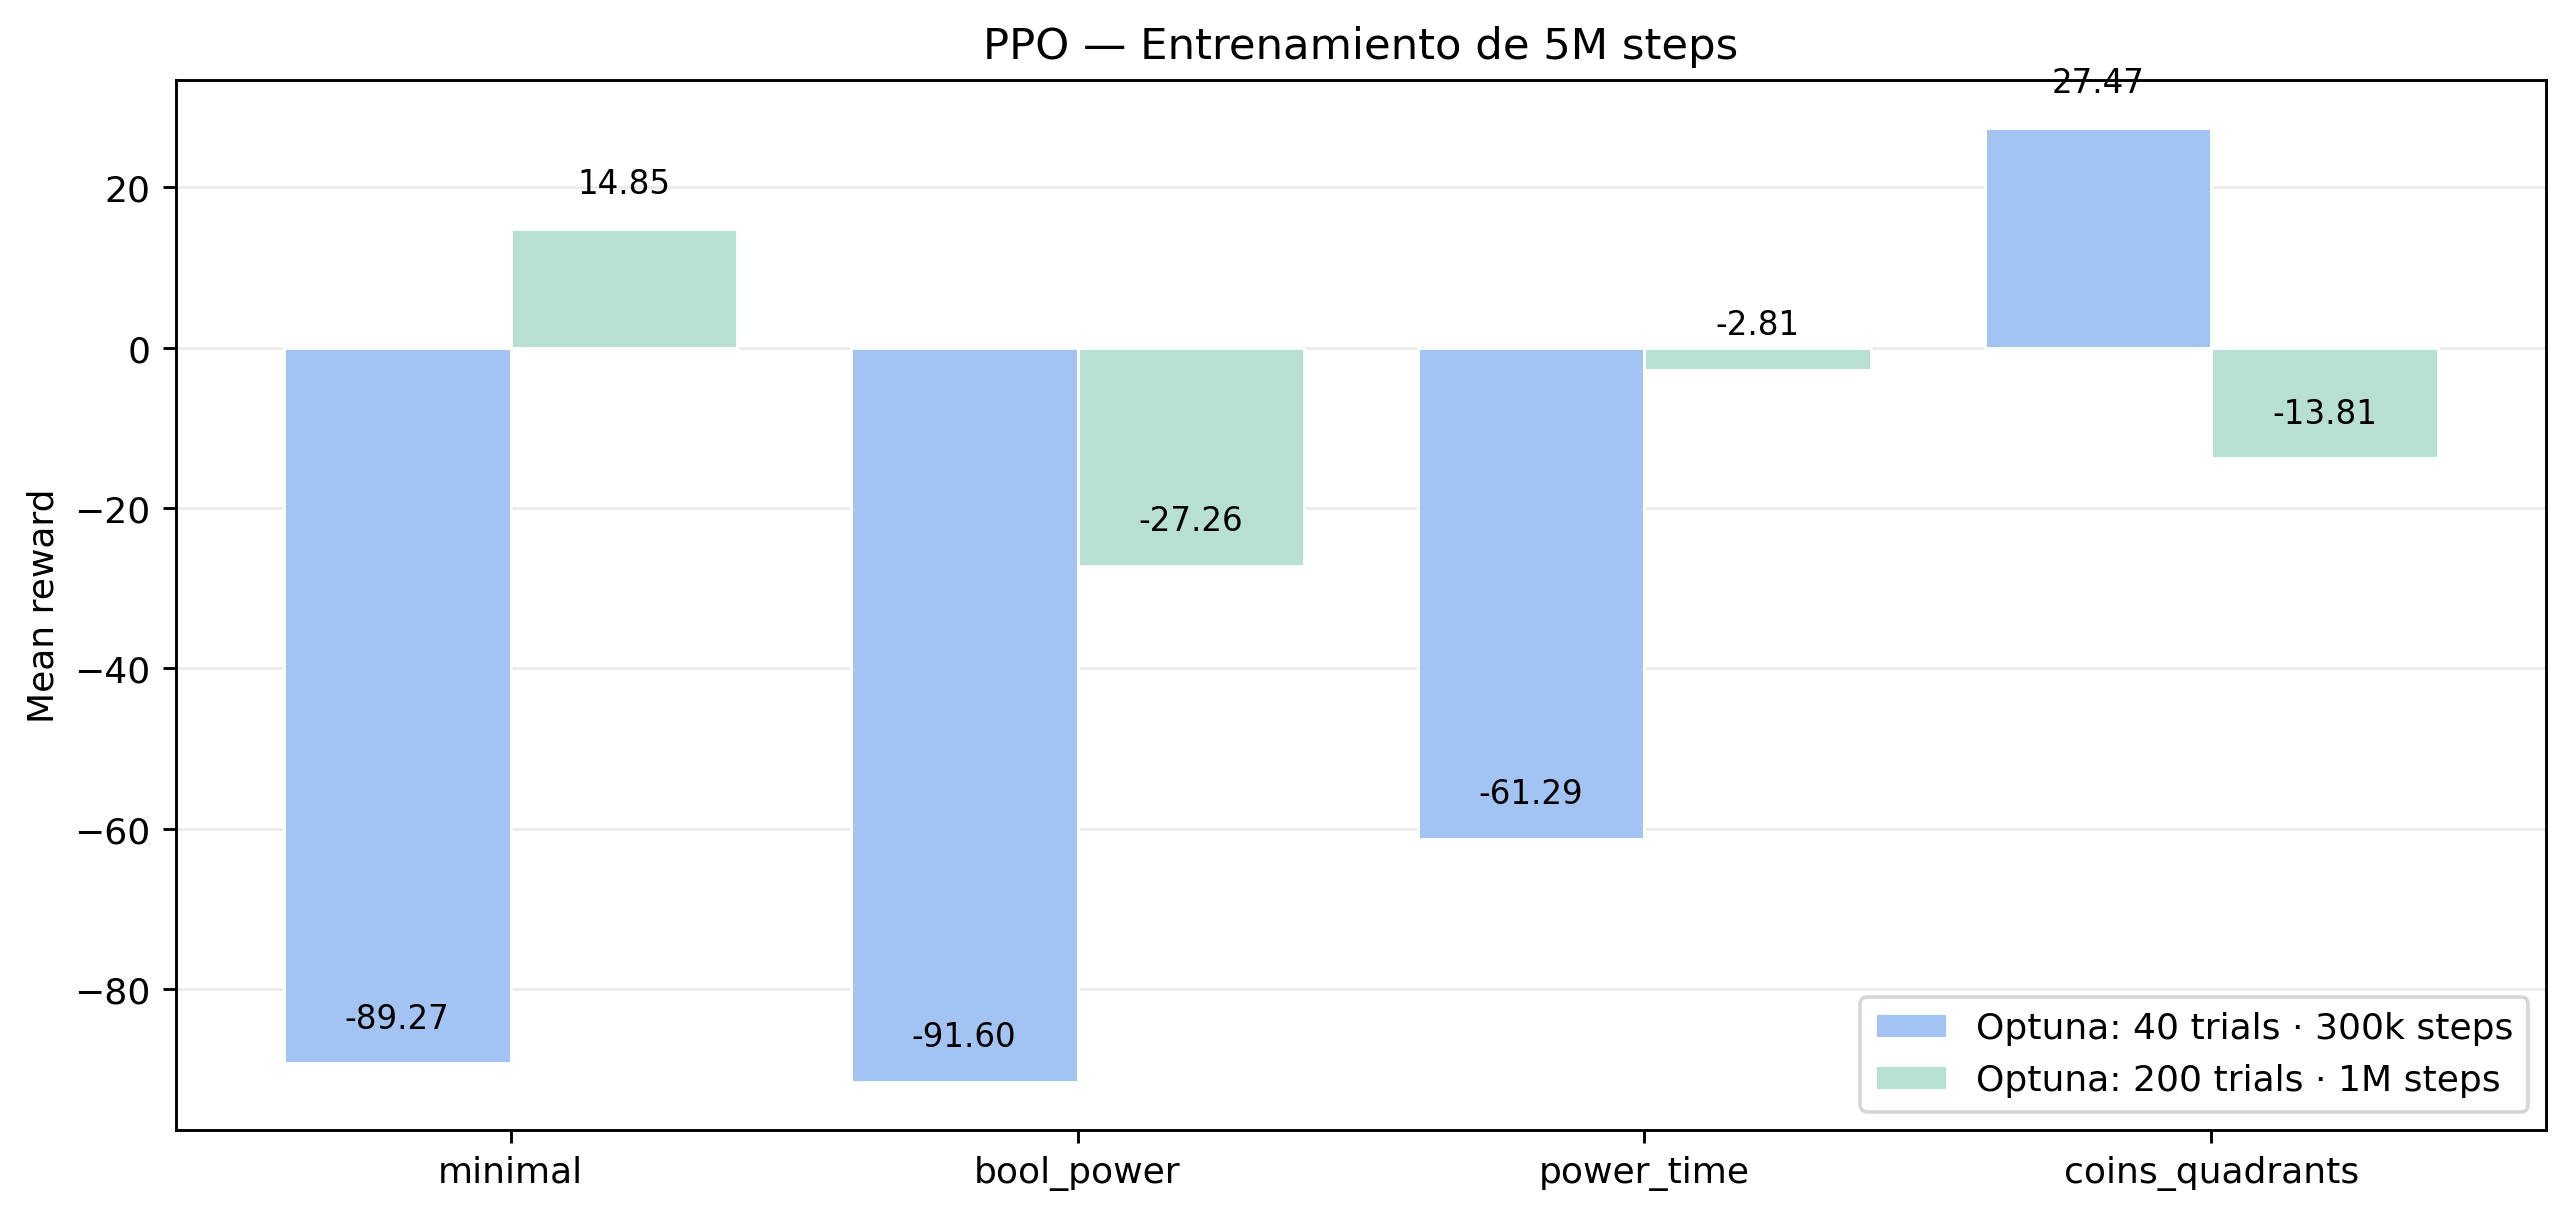
\includegraphics[width=0.5\textwidth]{./figs/graphics/ppo_optuna_mean_reward.png}
\caption{Mean reward con algoritmo de PPO entrenado con 5M de steps}
\label{fig:std_reward_a2c}
\end{figure}

\begin{figure}[h]
\centering
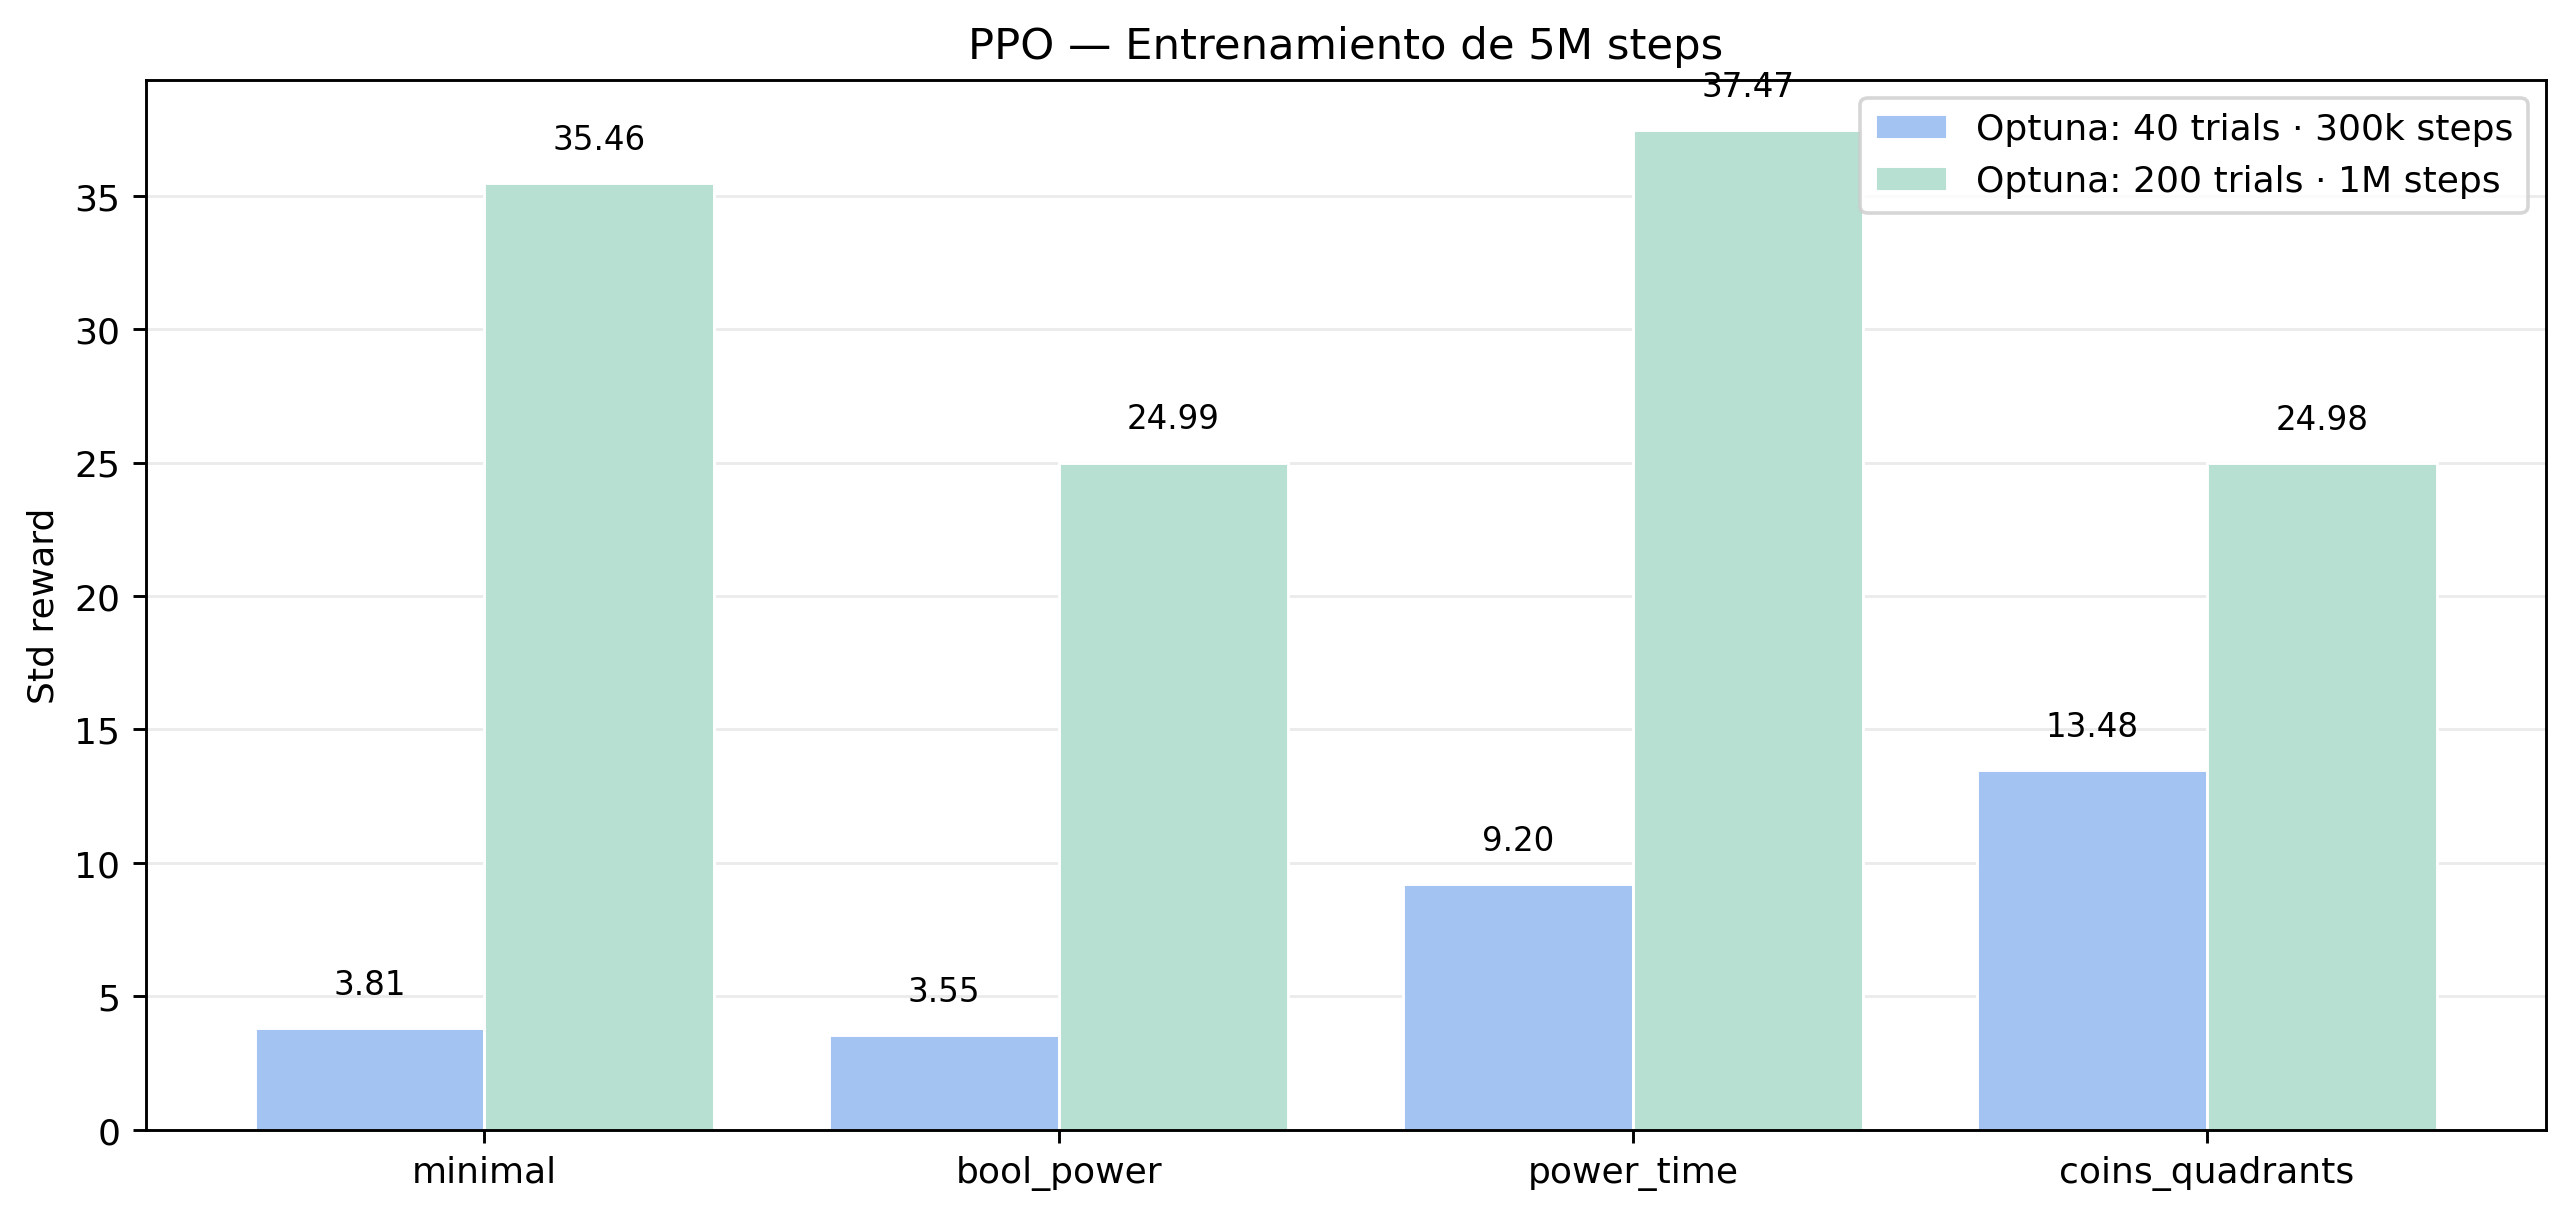
\includegraphics[width=0.5\textwidth]{./figs/graphics/ppo_optuna_std_reward.png}
\caption{Std reward con algoritmo de PPO entrenado con 5M de steps}
\label{fig:std_reward_a2c}
\end{figure}

El análisis de los distintos modos de observación revela que PPO se beneficia especialmente de representaciones del estado que incorporan información estructurada del entorno, como la distribución de monedas por cuadrantes. Sin embargo, el aumento de la complejidad del estado no garantiza una mejora sistemática del rendimiento, lo que refuerza la hipótesis de que existe un equilibrio óptimo entre simplicidad y riqueza informacional.

En conjunto, estos resultados posicionan a PPO como el algoritmo con mayor potencial en el entorno \textit{SimplePacmanEnv}, siempre que se disponga de un ajuste de hiperparámetros adecuado. Su capacidad para aprovechar observaciones más complejas y su rendimiento superior respecto a DQN y A2C lo convierten en un candidato especialmente relevante para el análisis comparativo presentado en las siguientes secciones.

\section{Comparación entre algoritmos}

En este apartado se comparan los resultados obtenidos con los tres algoritmos de Aprendizaje por Refuerzo evaluados en este trabajo: DQN, A2C y PPO. El objetivo es analizar sus diferencias en términos de rendimiento, estabilidad y eficiencia, manteniendo constantes las dinámicas del entorno, la función de recompensa y el protocolo de evaluación.

La comparación se realiza a partir de los mejores modelos obtenidos para cada algoritmo, seleccionados tras los correspondientes procesos de optimización de hiperparámetros y entrenados durante un número equivalente de pasos de entorno. De este modo, se garantiza que las diferencias observadas reflejen principalmente las características inherentes a cada algoritmo y su interacción con la complejidad del estado observado.

Desde el punto de vista del rendimiento absoluto, los resultados muestran que DQN es el algoritmo que alcanza los mayores valores tanto de recompensa media como de \textit{completion ratio}, especialmente a medida que aumenta la complejidad de la observación. PPO obtiene resultados competitivos en configuraciones concretas y muestra una elevada capacidad de adaptación cuando se dispone de una optimización exhaustiva de hiperparámetros, mientras que A2C presenta un comportamiento más estable pero claramente inferior en términos de progreso hacia la resolución del entorno. No obstante, ninguno de los algoritmos logra completar el entorno de manera sistemática, manteniendo tasas de éxito nulas en todas las configuraciones evaluadas.

\begin{figure}[h]
\centering
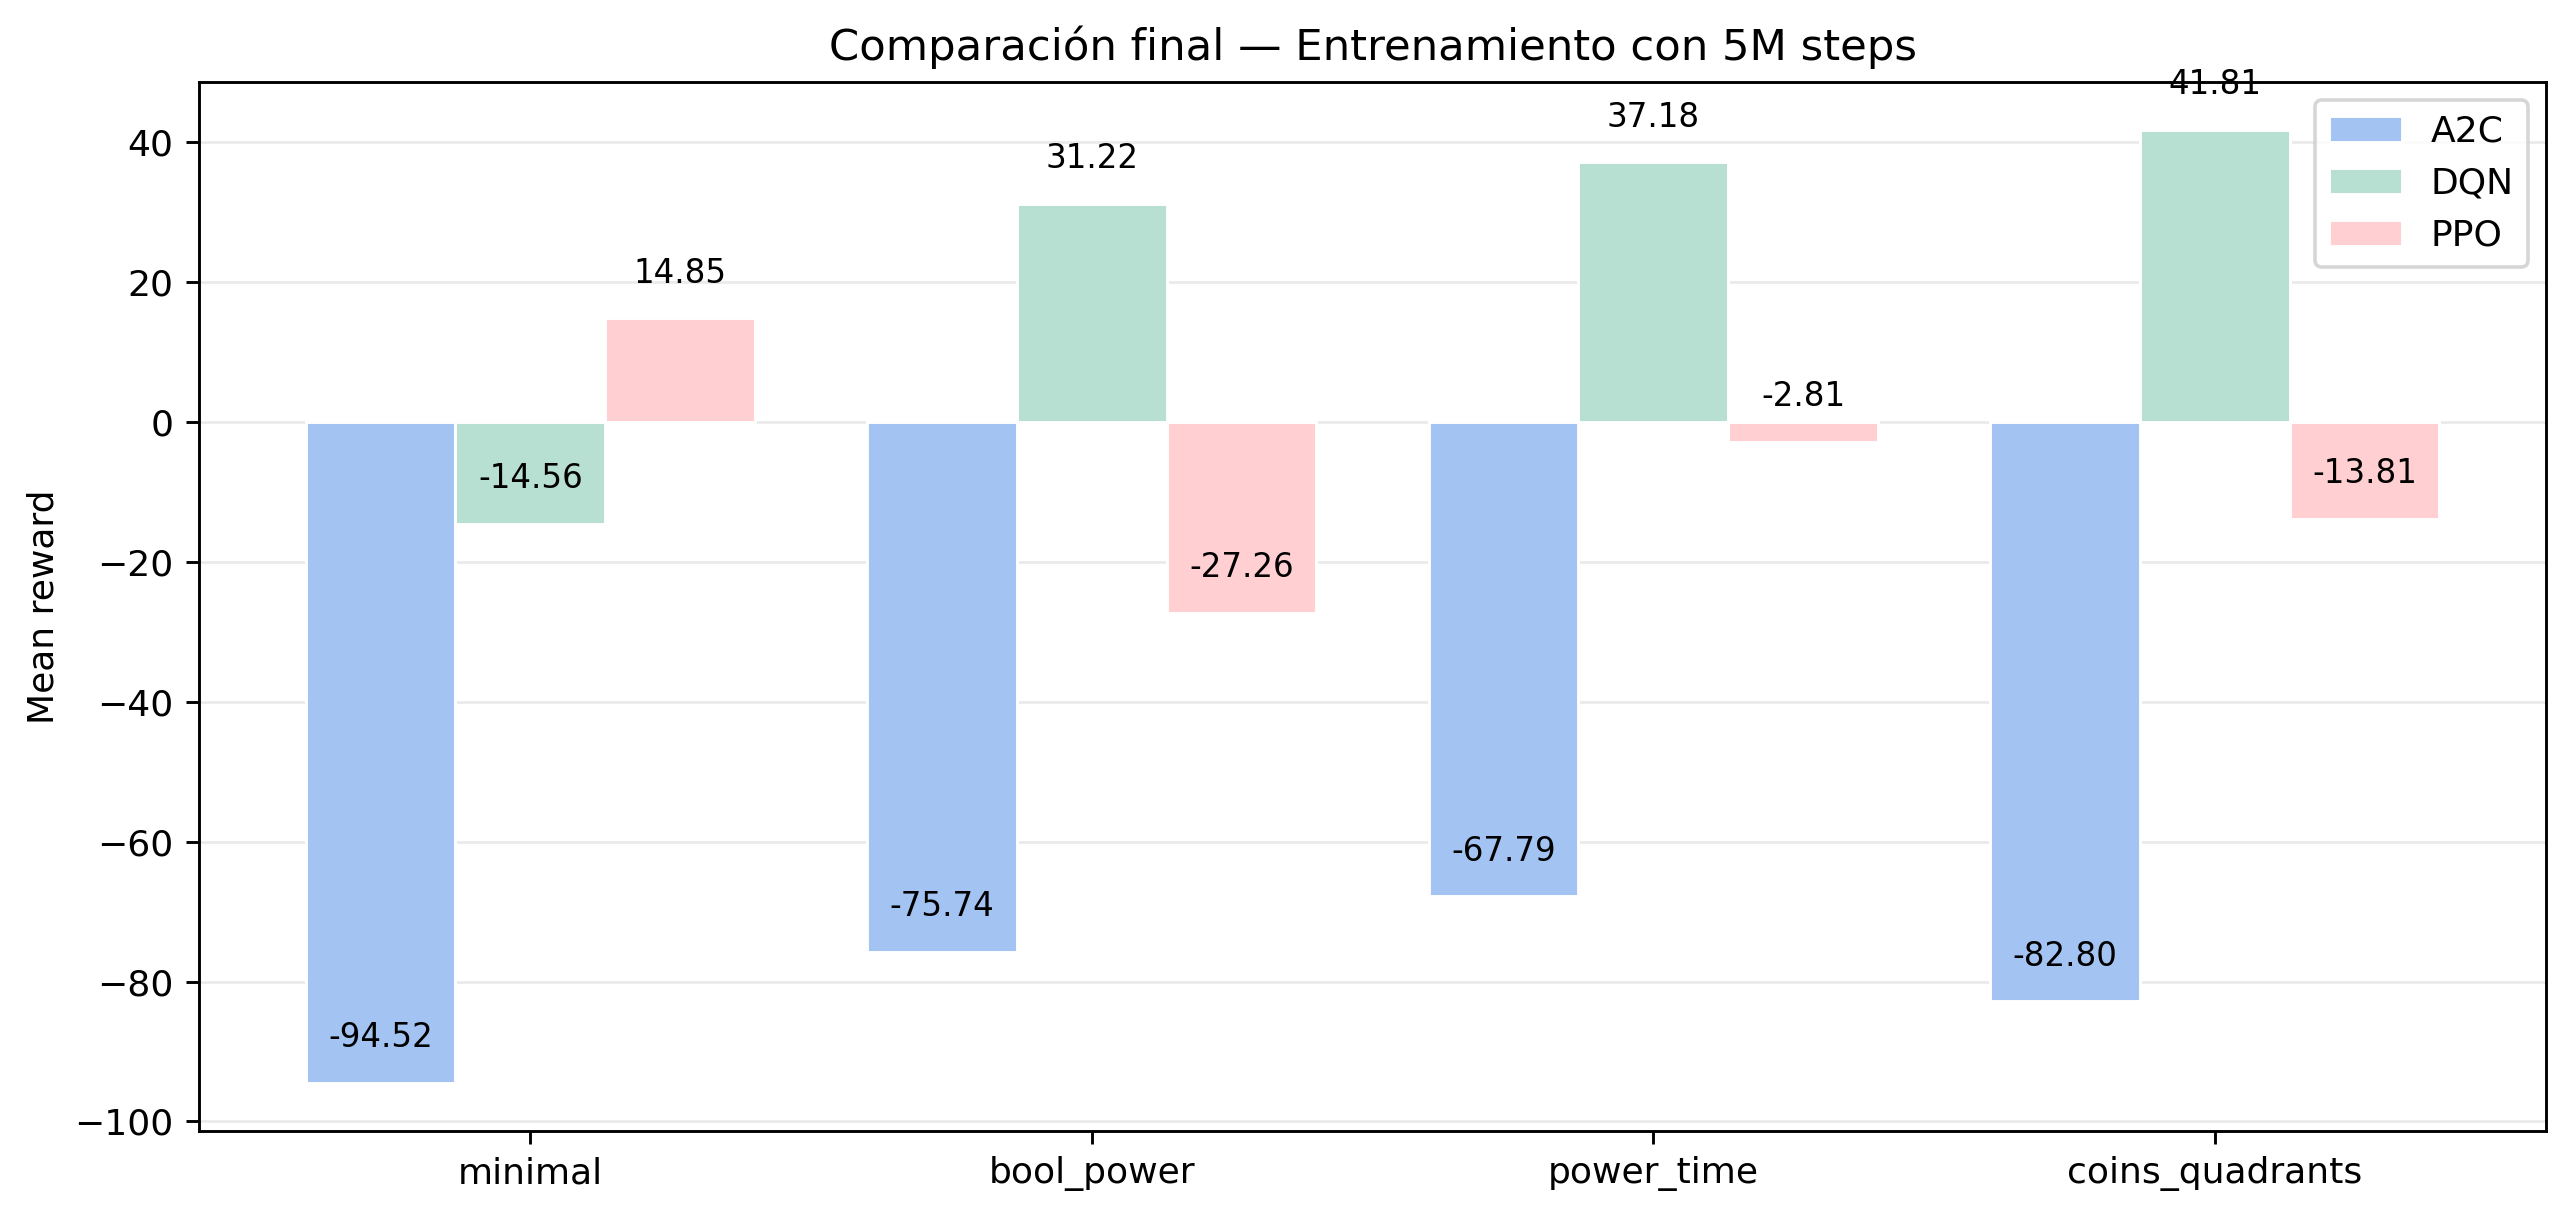
\includegraphics[width=0.5\textwidth]{./figs/graphics/final_algos_mean_reward.png}
\caption{Comparativa de mean reward entre algoritmos con 5M de steps}
\label{fig:std_reward_a2c}
\end{figure}

En términos de estabilidad del aprendizaje, se observan diferencias claras entre los algoritmos. DQN presenta una elevada variabilidad entre episodios, con grandes oscilaciones en la recompensa y episodios de duración prolongada, lo que indica políticas poco consistentes y sensibles a la configuración del estado. A2C, por el contrario, muestra un comportamiento más estable, con desviaciones estándar de recompensa menores y episodios más cortos, aunque a costa de un rendimiento global inferior. PPO se sitúa en un punto intermedio: logra recompensas y ratios de completado superiores, pero con una variabilidad notable, especialmente en configuraciones de observación más complejas.

\begin{figure}[h]
\centering
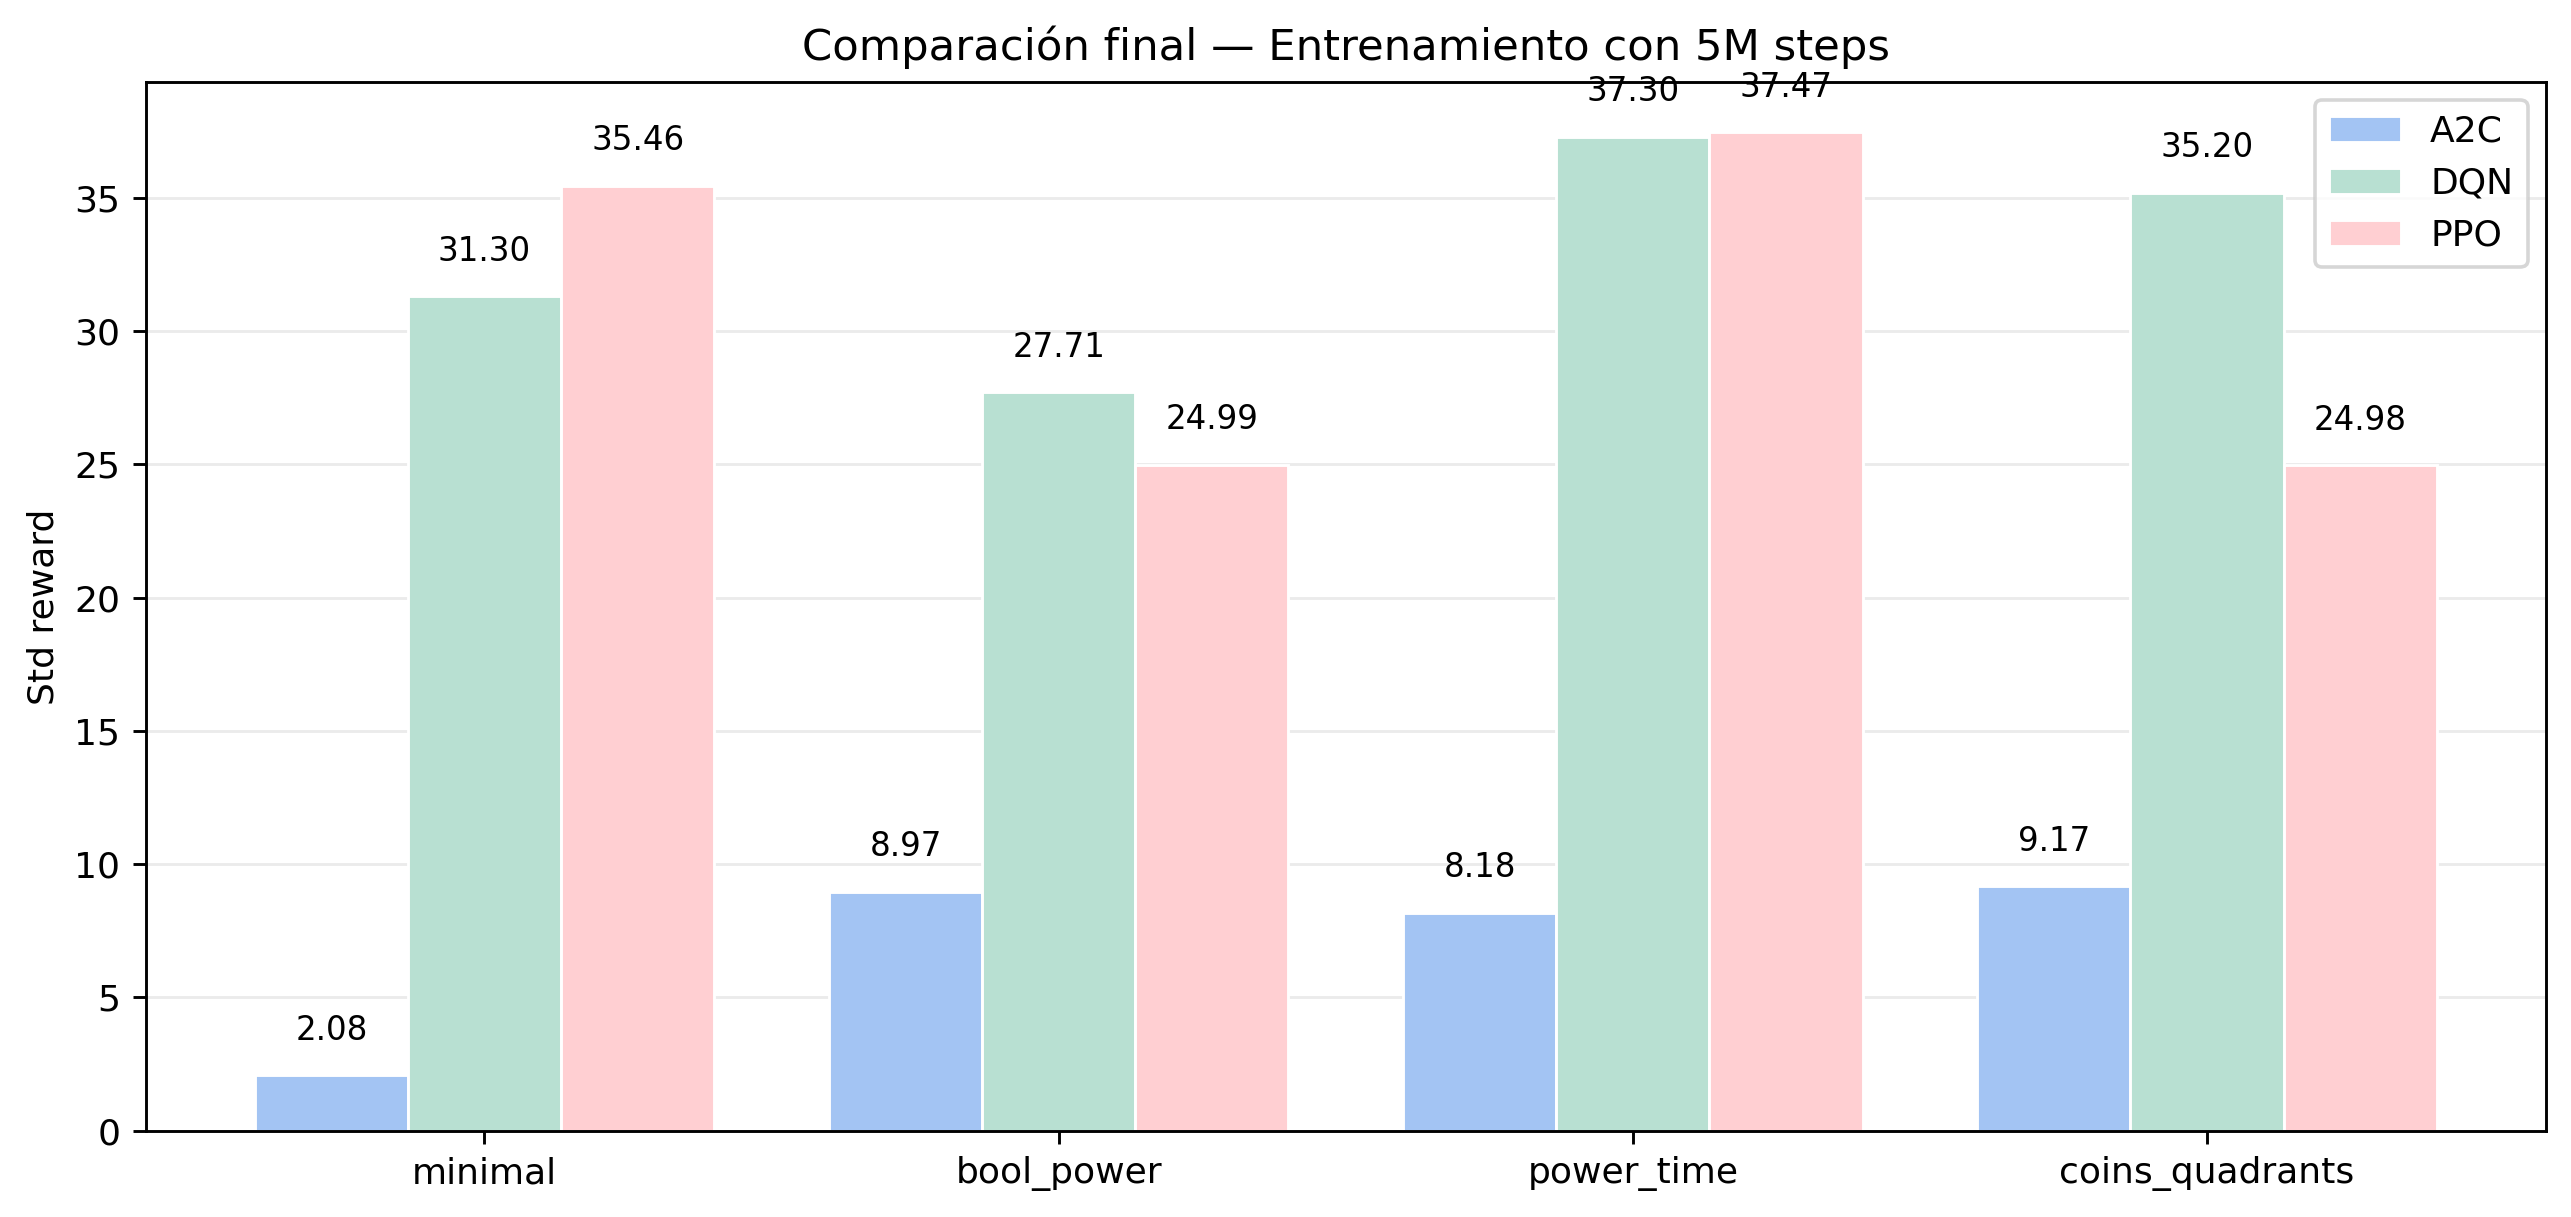
\includegraphics[width=0.5\textwidth]{./figs/graphics/final_algos_std_reward.png}
\caption{Comparativa de std reward entre algoritmos con 5M de steps}
\label{fig:std_reward_a2c}
\end{figure}

El coste computacional constituye otro factor diferenciador relevante. DQN resulta el algoritmo más costoso en términos de tiempo de entrenamiento y recursos necesarios para alcanzar un comportamiento razonablemente estable, lo que limita la viabilidad de realizar estudios exhaustivos de optimización. A2C presenta una mayor eficiencia computacional, permitiendo ejecutar un mayor número de experimentos y configuraciones en tiempos razonables. PPO, aunque más costoso que A2C, ofrece una mejor relación entre esfuerzo computacional y rendimiento final cuando se dispone de una optimización de hiperparámetros adecuada.

Finalmente, la sensibilidad a la complejidad del estado difiere de forma significativa entre algoritmos. DQN muestra un deterioro progresivo del rendimiento a medida que aumenta la dimensionalidad del espacio de observación, mientras que A2C tolera mejor observaciones más ricas, aunque sin traducir esta información adicional en mejoras sustanciales del rendimiento. PPO es el algoritmo que mejor aprovecha representaciones del estado más estructuradas, como la distribución de monedas por cuadrantes, aunque incluso en este caso el aumento de complejidad no garantiza una mejora sistemática.

\begin{figure}[h]
\centering
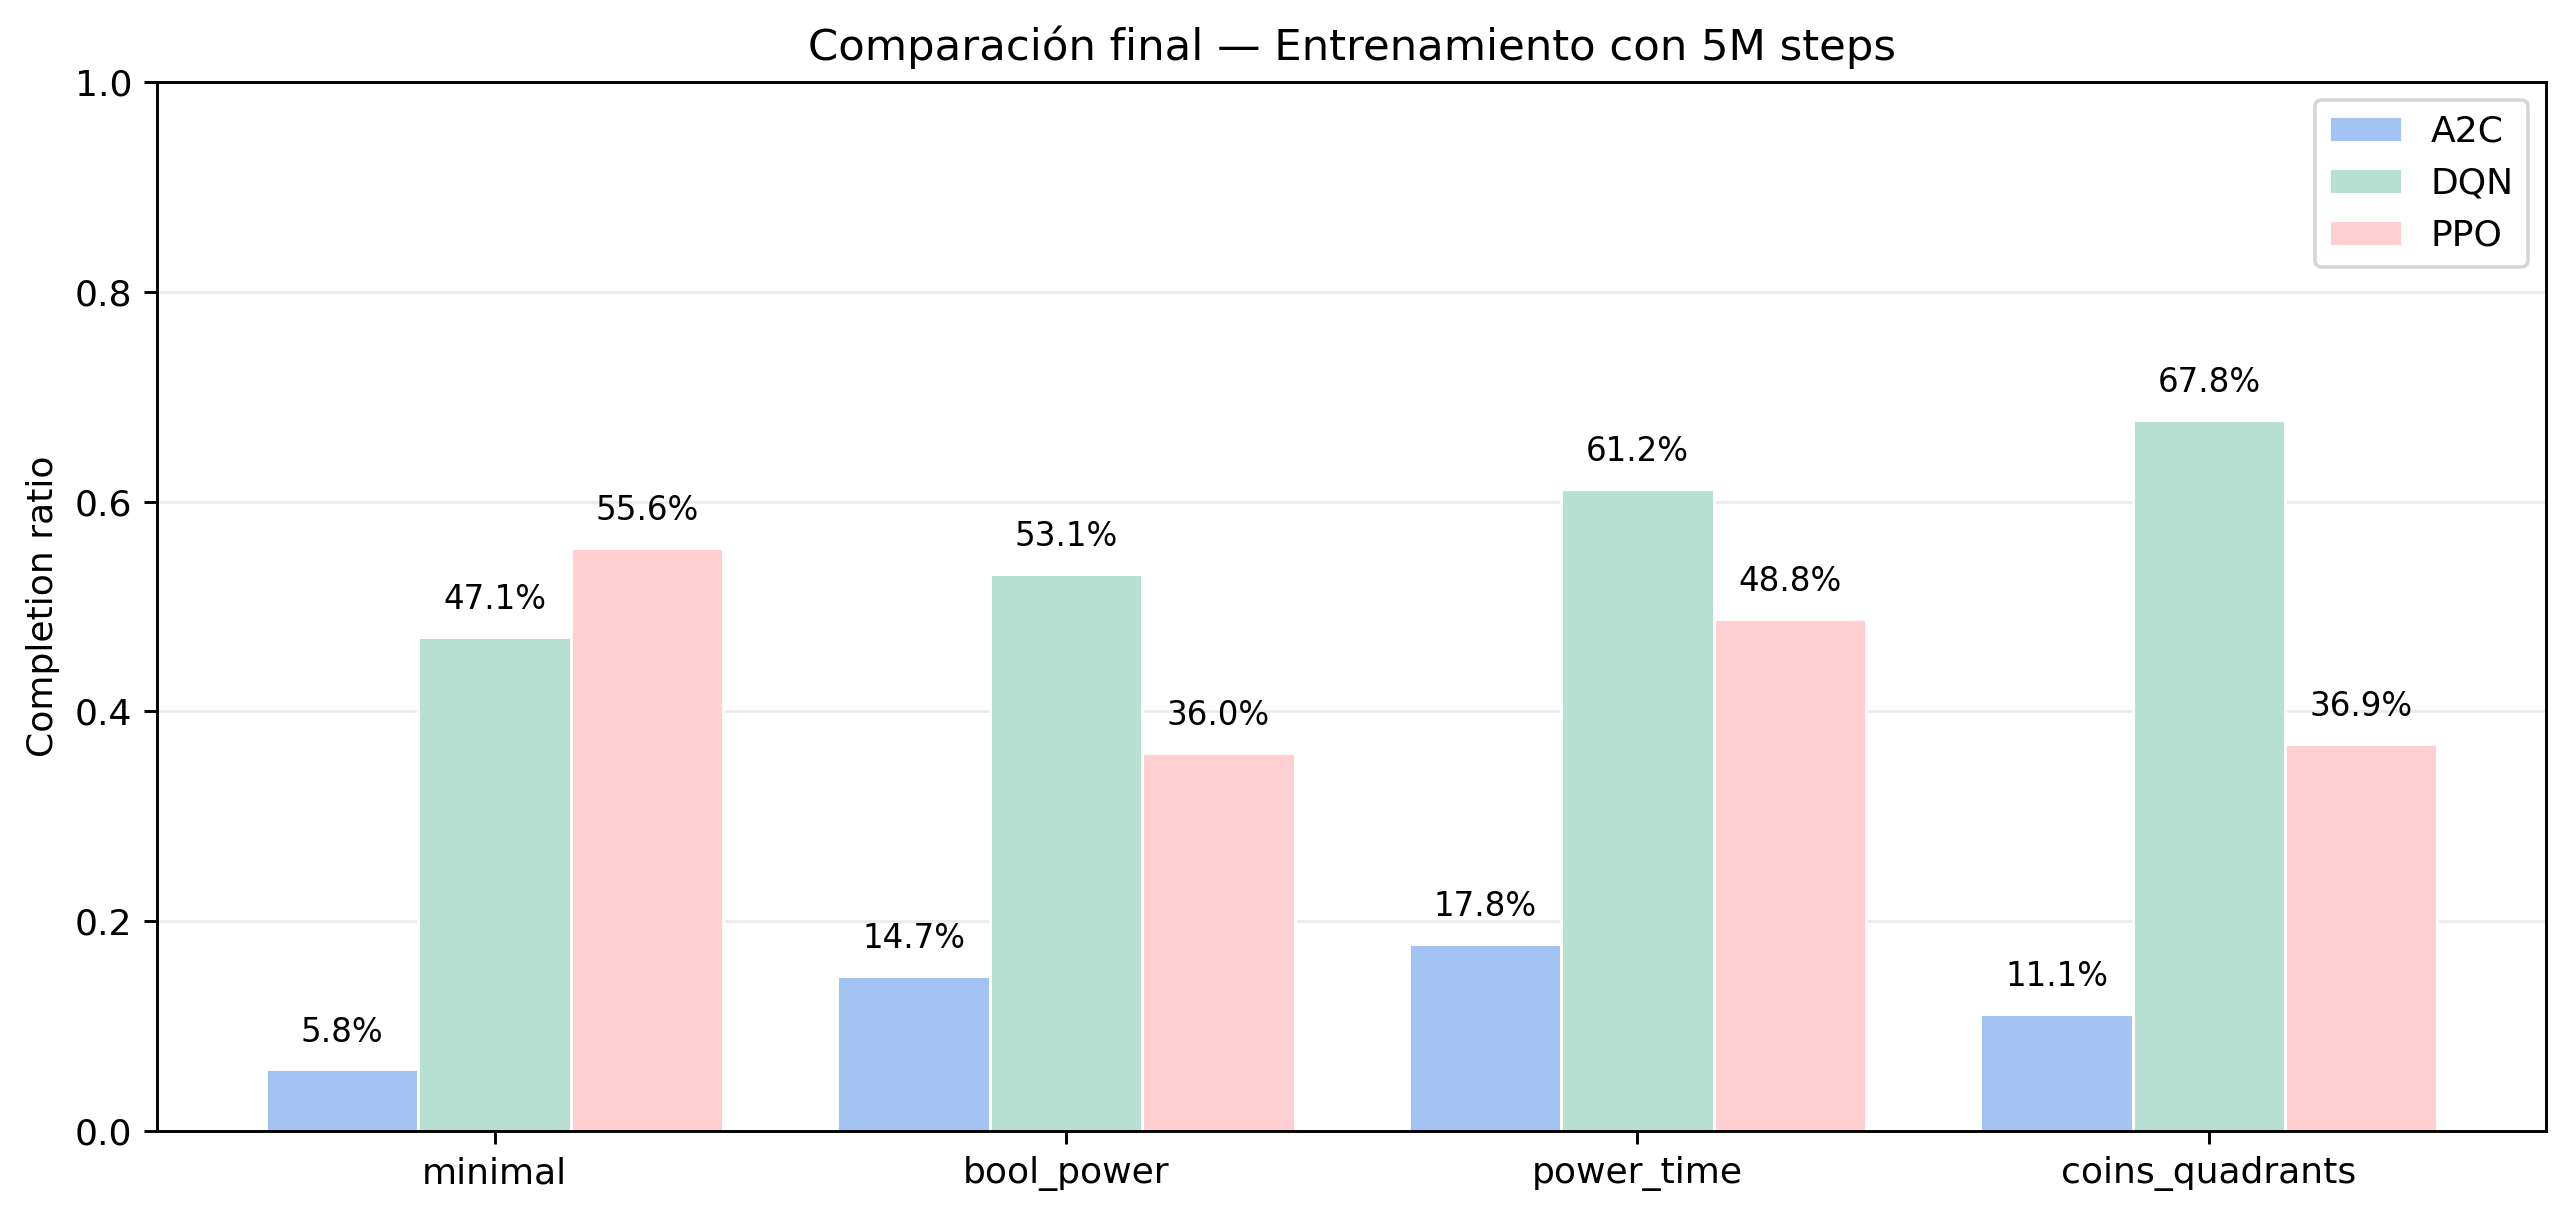
\includegraphics[width=0.5\textwidth]{./figs/graphics/final_algos_completion_ratio.png}
\caption{Comparativa de completion ratio entre algoritmos con 5M de steps}
\label{fig:std_reward_a2c}
\end{figure}

En conjunto, estos resultados evidencian que no existe un algoritmo universalmente superior, sino que el rendimiento depende tanto del método de aprendizaje como de la representación del estado. PPO emerge como el algoritmo más prometedor para el entorno estudiado, mientras que DQN y A2C presentan limitaciones claras en términos de estabilidad y capacidad de explotación de la información observacional.

\section{Impacto de la complejidad del estado}

El objetivo principal de este trabajo es analizar cómo la complejidad de la representación del estado influye en el rendimiento de los algoritmos de Aprendizaje por Refuerzo. En este apartado se integran los resultados obtenidos con DQN, A2C y PPO para evaluar de forma transversal el efecto de los distintos modos de observación definidos en el entorno \textit{SimplePacmanEnv}.

Para ello, se han considerado cuatro configuraciones principales de observación: observación mínima, observación con comodín binario, observación con temporizador de comodín y observación con distribución de monedas por cuadrantes. Estas configuraciones permiten incrementar progresivamente la cantidad y riqueza de la información accesible al agente, manteniendo constantes las dinámicas del entorno y el sistema de recompensas.

Los resultados muestran que la relación entre complejidad del estado y rendimiento del agente depende del algoritmo considerado. En particular, DQN presenta una tendencia clara de mejora progresiva del rendimiento a medida que se incorporan observaciones más informativas. Sin embargo, esta relación no se mantiene de forma uniforme en todos los algoritmos, lo que indica que el beneficio de estados más complejos está condicionado por la capacidad del método de aprendizaje para explotar dicha información adicional.

En los subapartados siguientes se analiza el comportamiento observado para cada tipo de representación del estado, integrando los resultados de los distintos algoritmos evaluados.

\subsubsection{Observación mínima}

La observación mínima proporciona al agente únicamente información básica sobre la posición del propio agente y del fantasma, omitiendo cualquier detalle sobre la distribución de monedas o el estado de los comodines. Esta configuración representa el nivel más bajo de complejidad del estado evaluado en el estudio.

En esta modalidad, los tres algoritmos muestran limitaciones claras en su capacidad de aprendizaje. DQN presenta recompensas medias bajas y un comportamiento altamente inestable, mientras que A2C obtiene los peores ratios de completado parcial del entorno entre todas las configuraciones evaluadas. PPO, aunque logra mejorar de forma notable el rendimiento cuando se optimiza de manera exhaustiva, tampoco alcanza una resolución consistente del entorno.

Estos resultados sugieren que una representación del estado excesivamente simplificada no proporciona la información necesaria para que el agente pueda planificar estrategias efectivas a largo plazo. En ausencia de información sobre la localización de objetivos, el aprendizaje se basa en comportamientos reactivos y locales, lo que limita la capacidad de completar la tarea.

\subsubsection{Observación con comodín binario}

La incorporación de una variable booleana que indica la activación de un comodín introduce información contextual adicional sin aumentar significativamente la dimensionalidad del estado. Este modo de observación permite al agente diferenciar entre situaciones de riesgo y ventaja temporal frente al fantasma.

Los resultados muestran que esta información adicional mejora el rendimiento respecto a la observación mínima en algunos algoritmos, especialmente en DQN y PPO, donde se observan incrementos en la recompensa media y en el ratio de completado parcial del entorno. Sin embargo, el impacto de esta mejora es limitado y no se traduce en una mayor tasa de éxito.

En el caso de A2C, la incorporación del comodín binario no produce mejoras significativas, lo que sugiere que este algoritmo requiere información más estructurada o rica para aprovechar de forma efectiva el contexto adicional. En conjunto, este modo de observación representa una mejora marginal, pero insuficiente para resolver las limitaciones estructurales del aprendizaje.

\subsubsection{Observación con temporizador de comodín}

El modo de observación que incluye el temporizador del comodín incrementa la complejidad del estado al introducir una dimensión temporal explícita. Esta información permite al agente anticipar la duración de su ventaja frente al fantasma y potencialmente planificar trayectorias más arriesgadas de forma controlada.

Este modo de observación muestra mejoras consistentes en A2C y PPO respecto a configuraciones más simples, alcanzando los mayores ratios de completado parcial del entorno en el caso de A2C. Sin embargo, el aumento de la complejidad también se acompaña de una mayor variabilidad en el rendimiento, especialmente en PPO, donde se observan episodios largos y comportamientos menos consistentes.

Estos resultados indican que la introducción de información temporal puede ser beneficiosa, pero también incrementa la dificultad del aprendizaje. La capacidad del algoritmo para explotar esta información depende en gran medida de su estabilidad y de la calidad del ajuste de hiperparámetros.

\subsubsection{Observación con distribución de monedas por cuadrantes}

La representación del estado mediante la distribución de monedas por cuadrantes proporciona una visión estructurada del entorno, capturando información espacial relevante sin recurrir a observaciones a nivel de celda. Este enfoque busca un equilibrio entre riqueza informacional y control de la dimensionalidad.

Los resultados experimentales muestran que este modo de observación es uno de los más efectivos, especialmente en el caso de PPO, donde se alcanzan los mayores ratios de completado parcial del entorno. Esta representación permite al agente inferir regiones de interés y planificar desplazamientos más coherentes, mejorando la eficiencia del aprendizaje.

No obstante, incluso en esta configuración, ninguno de los algoritmos logra completar el entorno de forma sistemática. Esto sugiere que, aunque la información espacial agregada resulta beneficiosa, sigue existiendo un límite en la capacidad de los algoritmos evaluados para integrar y explotar dicha información en un entorno con dinámicas adversas.

